\chapter{Образование}

\section{Про образование}

\textit{Источник: \url{https://bit.ly/3mQJ8N7}}

\textbf{Важность образования.}
Невозможно переоценить важность образования в современном мире. Образование стало ведущей силой технологического прогресса и тем самым всего развития человечества.

\textbf{Виды образования в России.}
В нашей стране есть разные виды образования: дошкольное, начальное, среднее и высшее.
Дошкольное образование охватывает ясли и детские сады. Там за детьми присматривают профессиональные няни и воспитатели. Часто их обучают читать и считать.

В России есть разные виды школ. Все школы начинаются с начального образования. Оно продолжается до 5 класса. Большинство учеников ходят в средние школы, другие идут в лицеи, гимназии, специализированные школы. Если ученики успешно оканчивают среднюю школу, они получают аттестат о среднем образовании. Он дает им возможность поступить в университет или академию, которые являются учреждениями высшего образования.

Учреждения высшего образования сейчас готовят специалистов, магистров и докторов. Диплом о высшем образовании позволяет найти более хорошую работу.

\textbf{Виды образования в других странах.}
В разных странах системы образования различны. В Британии три ступени образования. У Британцев есть начальная школа, средняя школа и высшее образование. Последнее включает профессиональное и собственно высшее образование.
В США система образования очень децентрализована. Это означает, что каждый штат имеет свои законы об образовании. Как правило, там есть начальные школы (6-11 лет), средние школы (11-15 лет) и старшие школы (9-12 классы). Есть несколько способов продолжить образование: университеты, колледжи, местные колледжи, технические и профессиональные школы.

\clearpage
\section[Что мешает хорошо обучаться]{Ученые из России и Швеции выяснили, что мешает хорошо обучаться}

\textit{Источник: \url{https://trends.rbc.ru/trends/education/62a849179a7947b0cc4329a4?from=mainpage}}

Ученые из МГУ, Сколтеха и Стокгольмского университета выяснили, от чего зависит способность к обучению. Рассказываем, что нужно об этом знать

\textbf{Что происходит}

В организме белок синтезируется с помощью рибосом в ядре и цитоплазме, либо в митохондриях. Первый способ изучен хорошо, второй --- недостаточно.

Два года назад ученые из МГУ открыли два фермента --- белковых соединения, которые участвуют в сборке рибосом в митохондриях. Затем ученые из Стокгольмского университета выделили митохондрии с недостроенными рибосомами, определили их структуру и показали процесс их сборки. Выяснилось, что в этих клетках были неактивными ферменты метилтрансферазы.

Чтобы проверить влияние неактивных ферментов на организм, ученые из МГУ вырастили мышей с такими ферментами. Затем провели эксперимент: посадили животное в ящик с несколькими выходами, где только один ведет в домашнюю клетку, остальные --- в тупик. Если нормальная мышь запоминает правильный выход и в следующие разы бежит именно туда, то мышь с неактивными ферментами не запоминает правильный путь и каждый раз ищет его заново.

Таким образом, пришли к следующему выводу. Если ферменты метилтрансфераза неактивны, то работа митохондрий нарушается, и в клетки перестает поступать энергия. Из-за этого мышцы становятся слабее, а интеллектуальные способности снижаются.

\textbf{Что это значит}

Ученые из МГУ уже исследовали нарушения в работе митохондрий. В мае 2022 года они пришли к выводу, что нарушение работы этих органелл приводит к старению. Это происходит из-за того, что с возрастом появляется все больше нарушений в работе митохондрий, и клетки не успевают их устранять. Чтобы уменьшить число поломок и замедлить старение, согласно исследованиям ученых, нужно соблюдать диету.

По словам руководителя отдела разработки ДНК-тестов в компании MyGenetics Валерия Полуновского, чем лучше работают митохондрии в организме человека, тем лучше функционирует тело и мозг. А чтобы число митохондрий в клетках стало больше, нужно заниматься спортом.

\clearpage
\section{Система Лейтнера}

\textit{5 шагов, позволяющих выучить что угодно}

\textit{Источник: \url{https://4brain.ru/blog/sistema-lejtnera/}}

\begin{wrapfigure}{l}{0.5\textwidth}
    \begin{center}
        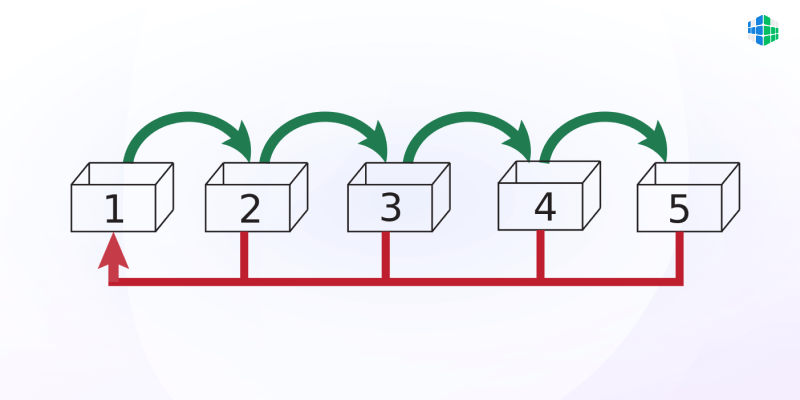
\includegraphics[width=0.49\textwidth]{img/sistema-lejtnera.png}
    \end{center}
    \caption{Система Лейтнера: 5 шагов, позволяющих выучить что угодно}
\end{wrapfigure}
Как часто вам приходится жаловаться на память? Как часто вам нужно что-то запомнить, а оно никак не запоминается? И как быстро вам надоедает все это повторять настолько, что вы решаете обойтись без этих знаний?

С подобной ситуацией сталкивается около 80\% людей, изучающих, например, иностранный язык. И как раз в помощь им была создана система Лейтнера. Однако впоследствии оказалось, что она пригодна для запоминания любой другой информации. Что же это за система такая?

\textbf{Волшебные карточки Лейтнера}

Основой системы Лейтнера являются так называемые флэш-карточки, на которых записывается информация для запоминания. Карточки могут быть обычными бумажными либо электронными.

За основу бумажной версии можно взять обычные каталожные карточки, которые можно увидеть в любой традиционной библиотеке, где есть каталоги – алфавитный, систематический, топографический. Как вариант, можно вырезать карточку удобного лично вам размера из плотной бумаги или тонкого картона.

Лайфхак для офисов и издательств – не выбрасывайте оставшиеся невостребованными карманные календарики за прошлый год. На светлом фоне можно писать черным маркером, а такие карточки будут выглядеть интереснее и веселее, чем обычные, сделанные из одноцветной бумаги.

Электронные карточки можно сделать в любом мобильном приложении для создания заметок или же воспользоваться специальным софтом. Для русскоговорящих пользователей можно рекомендовать мобильное приложение Brainscape или онлайн-программу Quizlet, также имеющую версии для iOS и Android.

Принцип использования бумажных и электронных карточек идентичен. Разница лишь в том, каким способом вы будете «тасовать колоду»: перелистывая экран или перекладывая карточки из одной стопки в другую.

\textbf{Как пользоваться карточками}

Каждый из нас замечал, что даже самое банальное «не получается» имеет свои градации: не очень получается, не всегда получается, не получается от слова «совсем». Если воспользоваться традиционным линейным способом заучивания, весь материал придется проходить каждый раз от начала до конца, будь то список новых слов по английскому, набор формул по физике или даты исторических событий.

Система Лейтнера позволяет не тратить время на повторение уже выученного материала, даже если он идет в связке с пока неизученным. Эта система удобна тем, что можно сосредоточиться только на том, что пока никак не запоминается, и регулировать частотность повторений по мере усвоения. Как это работает?



Алгоритм использования флэш-карточек:
\begin{enumerate}
    \item Распределяем весь изучаемый в данный момент материал по карточкам в режиме 1 карточка = 1 единица информации.
    \item Карточки с информацией, которую не получается запомнить совсем, складываем в первую колоду и повторяем ежедневно.
    \item Карточки с информацией, которую вы помните фрагментарно, помещаете во вторую колоду и повторяете через день.
    \item Карточки с информацией, которую вы иногда забываете или не всегда можете быстро вспомнить, помещаете в третью колоду и повторяете раз в три дня.
    \item По мере освоения материала карточки из первой колоды перекладываете во вторую, а затем в третью колоду.
\end{enumerate}

Такой подход называется методом интервальных повторений, т.е. повторений с определенными оптимальными для достижения результата интервалами. Не обязательно перечитывать всю колоду за один раз. Прочитайте столько, сколько успеваете, пока едете на работу, стоите в очереди, помешиваете кашу на медленном огне. Таких «бесполезных пятиминуток» может быть несколько в течение дня, и в сумме набегают те же 45 минут, что нужны для полноценного урока.

Теперь чуть подробнее о единицах информации. Это может быть, например, слово на английском – транскрипция – перевод на русский. Или формула по физике с расшифровкой переменных, внесенных в формулу. Или дата и название исторического события. Такой подход идеален для школьников в возрасте до 12-13 лет, которым сложно воспринимать сразу большой объем сведений.

Студенты, старшеклассники и взрослые могут расходовать площадь карточки более экономно и записывать на одну карточку сразу 2-3 связанные единицы информации. Например, три формы глагола в английском, две формулы из раздела «Кинематика» для расчета средней скорости движения и средней скорости при неравномерном движении, даты первого, второго и третьего раздела Польши в 18 столетии. Само собой, для трансфера карточки в следующую колоду нужно освоить все слова, формулы, даты с карточки.

К слову, при использовании электронных карточек вы можете получать рекомендации, сколько времени вам потребуется для запоминания той или иной информации и как часто нужно ее повторять. В частности, эта функция есть в приложении Brainscape. Вам требуется на старте самостоятельно оценить свой уровень знаний по каждой карточке от 1 до 5, и приложение выдаст свои рекомендации для дальнейшего изучения материала.

Английский, физику и историю мы взяли исключительно для примера. На самом деле, область применения карточек намного шире.

\textbf{Область применения системы Лейтнера}

Мы начали с того, что изначально данная система была разработана Лейтнером для изучения иностранного языка. Себастьян Лейтнер был журналистом, поэтому знание языков было для него профессиональной необходимостью.

Процесс изучения языка был адаптирован под существующие обстоятельства, т.е. высокую мобильность профессии журналиста, когда из-за постоянных разъездов и командировок не получается выделить фиксированное время для занятий.

Набор флэш-карточек с новыми словами, формами глаголов, местоимений, причастий, деепричастий всегда можно взять с собой. Небольшой набор легко поместится в карман мужского пиджака, а две-три стопки не займут много места в сумке. К слову, для изучения иностранных языков можно приобрести готовые карточки.

Точно так же с помощью флэш-карточек можно готовиться к экзамену по любому предмету в школе и вузе, докладу на семинаре или конференции, запоминать расположение нот и варианты аккордов на грифе гитары, разучивать длинную песню, разделив ее на куплеты, бридж и припев, а в особо сложных случаях переписав на карточки построчно.

Так же с помощью карточек можно развивать память и остроумие, поместив на них короткие шутки, анекдоты, изречения по разным поводам. Если регулярно повторять шутки и анекдоты, которые имеют свойство забываться, через какое-то время ваш мозг будет моментально реагировать на подходящую ситуацию, где можно блеснуть остроумием и выдать актуальный юмор.

Многим эта система так нравится, что они готовы заменить ею весь учебный процесс. Стоит ли это делать? Давайте подумаем.

\textbf{Система Лейтнера: в придачу или вместо?}

Тут хочется вспомнить известную поговорку: все хорошо в меру. Конечно же, система Лейтнера не может полностью заменить лекции, семинары и уроки хотя бы потому, что на семинарах и лекциях можно получить обратную связь преподавателя.

Разумеется, система Лейтнера не может заменить систематизированный курс по какой-либо специализации, будь то приемы оказания первой медицинской помощи или основы компьютерной грамотности. Карточки лишь носители единиц информации, а полностью овладеть знаниями можно, только когда вы получаете систематизированный курс лекций в нужной последовательности и учитесь применять полученные сведения на практике.

По этой же причине система не может стать альтернативой получению среднего или высшего образования, даже если на карточки перенести все формулы и даты по всем предметам. Однако система Лейтнера может существенно дополнить традиционные методы обучения, облегчить процесс усвоения и сэкономить время на изучение материала.

Как было сказано выше, пользование флэш-карточками вовсе не требует выделения фиксированного времени в вашем распорядке дня, и вы можете заполнить карточками любой пустой отрезок дня, когда не предвидится ничего более важного и интересного.

Если такой не заполненный полезными делами промежуток времени оказался слишком большим, вы можете повторить информацию из всех трех колод, а потом пойти по кругу, вернувшись к первой стопке. Это будет исключительно вам на пользу и станет отличной проверкой функциональности вашей кратковременной памяти. Вы сами сможете увидеть, с какой скоростью вы запоминаете или забываете информацию и, возможно, откорректировать методы самообразования в дальнейшем. Теперь подытожим все преимущества системы.

Преимущества системы Лейтнера:
\begin{enumerate}
    \item Простота и доступность.
    \item Возможность реализовать в бумажном или электронном формате по выбору.
    \item Возможность использования везде и всюду.
    \item Применимость для разных областей знания.
    \item Пригодность для подготовки к экзаменам по любым предметам.
    \item Пригодность для запоминания любой информации, которую можно разбить на короткие логические блоки.
    \item Развитие памяти – оперативной, среднесрочной и долгосрочной.
\end{enumerate}

К слову, с развитием памяти и техник запоминания информации вам может помочь наш курс «Мнемотехники», где вы освоите полезные лайфхаки, как быстро и надежно запоминать имена, даты, лица, термины, иностранные слова и все, что вам нужно. В качестве бонуса по окончании курса вы получите новый уровень развития ассоциативного мышления и научитесь придумывать рифмы к любым словам, требующим запоминания.

Так что желаем вам свежих знаний, полезных сведений, новой информации и ждем вас на нашем курсе, где научим все это запоминать. Поделитесь ссылкой на курс у себя на страничке в соцсетях – так вам будет легче вспомнить, где именно стоит искать этот курс, когда вы будете готовы начать учиться. Удачи!

\clearpage
\section{Метод изучения языков Китайгородской}

\textit{Источник: \url{https://4brain.ru/}}

\begin{wrapfigure}{l}{0.5\textwidth}
    \begin{center}
        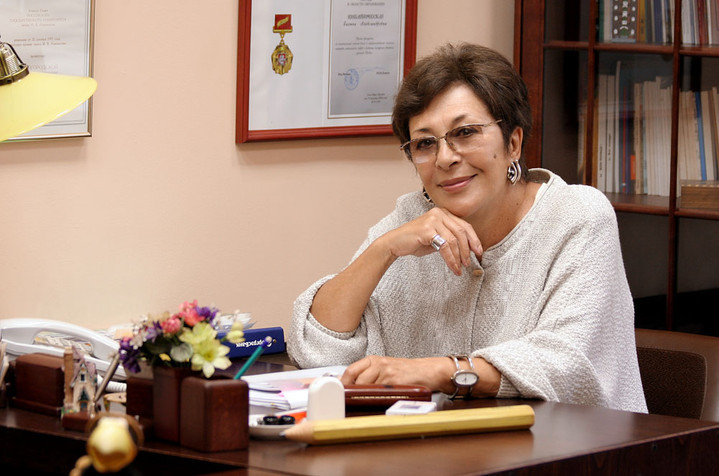
\includegraphics[width=0.49\textwidth]{img/kitaigorodskoi.jpg}
    \end{center}
    \caption{Китайгородская, Галина Александровна}
\end{wrapfigure}
С каждым днём в сфере образования появляются какие-то новые \ed{разработки}{разработка}{development}, программы, \explain{обучающие методики}{teaching methods} и другие всевозможные \ed{н\'{о}вшества}{н\'{о}вшество}{innovation}. Старые, же, или, как ещё их можно назвать, традиционные, если уж и не забываются, то просто отодвигаются на задний план по причине потери своей \ed{актуальности}{актуальность}{relevance} и малой эффективности. И эта тенденция наблюдается во всех направлениях, по которым происходит обучение, в том числе и в изучении иностранных языков.

Большинство традиционных методик обучения иностранным языкам сейчас \explain{подвергается}{undergoes; is subjected to} жёсткой критике, т.к. многие специалисты считают, что обучать им современных детей, да и взр\'{о}слых тоже, следует по ин\'{о}му пут\'{и}. А представление о прив\'{ы}чных мет\'{о}диках обучения складывается прим\'{е}рно такое:
\begin{enumerate}
    \item Огромное количество тр\'{у}дных грамматических правил, которые необходимо заучивать
    \item Десятки листов со словами, которые также нужно заучивать
    \item Объёмные неинтересные тексты, которые нужно читать, переводить и пересказывать
\end{enumerate}

Как вы сами считаете, нужно ли продолжать применять такие м\'{е}тоды в современных образовательных учреждениях? Наверняка, вы скажете, что лучше найти нечто более интересное и эффективное, что оказывало бы на учащихся большее стимулирующее воздействие, и помогало бы им гораздо быстрее осваивать лексику, грамматику и фонетику того языка, который они изучают.

И на сег\'{о}дняшний день исследователи \explain{выделяют}{identify} два основн\'{ы}х инновационных пути изучения языков, которыми являются:
\begin{enumerate}
    \item Применение методов изучения иностранных языков, осн\'{о}вывающихся на эффекте сверхзапоминания, когда восприятие и усвоение информации происходит без её критического осмысл\'{е}ния;
    \item Применение нетрадиционных методов, которые подразумевают ускоренное и максимально интенсивное обучение иностранному языку, где теоретическая база является минимальной или её вообще нет, а \explain{основной уп\'{о}р}{main emphasis} д\'{е}лается на практике, т.е. на разговорной речи в процессе жив\'{о}го общения.
\end{enumerate}

Базой об\'{о}их этих путей являются принципы суггестологии, которые б\'{ы}ли разработаны болг\'{а}рским педагогом и псих\'{о}логом Геогрием Лозановым. Ст\'{о}ит сказать, что суггестология является наукой, посвящённой раскрытию скрытого потенциала человека, и активизирующей его подсознательные ресурсы. В качестве примера можно назвать м\'{е}тод всем известного «25 кадра», а также обучение во сне. И как раз одним из м\'{е}тодов обучения иностранным языкам, которые основываются на принципах суггестологии, является метод Галины Александровны Китайгородской.

\textbf{Метод Г. А. Китайгородской}

Метод Г. А. Китайгородской, который также называют м\'{е}тодом «Активизации рез\'{е}рвных возможностей личности и коллектива», нельзя назвать новым, т.к. он был разработан свыше 35 лет назад, однако он считается исключительно \ed{нов\'{а}торским}{нов\'{а}торский}{innovative} и уже ставшим классическим в области интенсивного обучения.

Важно также сказать, что именно Галиной Александровной Китайгородской была создана единственная в России научная система интенсивного обучения иностранным языкам, а также был введён сам термин «интенсивное обучение». И с момента создания этой системы её эффективность была оценена огромнейшим количеством людей, которые в рек\'{о}рдно короткие сроки овладели иностранными языками.

Отличие м\'{е}тода Китайгородской от традиционных заключается в том, что он \explain{з\'{и}ждется}{is based on} на психологических резервах личности и коллектива при \ed{целенаправленной}{целенаправленный/-ая}{purposeful; targetted} манипуляции социально-психологическими процессами \ed{межличностного}{межличностный}{interpersonal} группового взаимодействия, благодаря чему учащиеся за совершенно мизерное время очень легко и продуктивно перерабатывают большие объёмы новых знаний.

Ключевое место в системе интенсивного обучения занимает термин «активизация» --- процесс, который направлен на достижение человеком активности и стабилизацию данного состояния. В своей изначальной интерпретации понятие «интенсивность» рассматривается как «напряжённость», а именно: состояние активности в конкретный момент времени. Точно также следует и трактовать понятие «интенсивного обучения» в рамках системы Г. А. Китайгородской – оно должно пониматься как динамизм, активное взаимодействие педагогов и группы учащихся, учащихся друг с другом, активизация процессов \ed{познания}{познание}{knowledge; cognition}, ресурсов памяти, воображения и внимания.

Тот ученик, который устал, засыпает на занятиях и нисколько не заинтерес\'{о}ван в своём обучении, не способен \explain{надлеж\'{а}щим \'{о}бразом}{properly} воспринимать большие объёмы информации и \explain{всецело}{wholly; entirely} отдаваться общению со своими партнёрами по обучению. А методика Китайгородской спос\'{о}бна привести учащегося в такое состояние, в котором он будет максимально \explain{\'{у}мственно}{mentally} и нередко даже физически активен, по причине чего будет обесп\'{е}чен самый высокий показатель интенсивности процесса обучения. Если говорить несколько проще, путь овладения человеком иностранным языком, согласно системе Китайгородской, очень \explain{схож}{similar} с тем путём, идя по которому ребёнок осваивает свой родной язык.

Сначала учен\'{и}к двигается вперёд по различным стадиям формирования способности к речи, начиная с интонационной, затем переход\'{я} к лексико-грамматической, а после --- к синтаксической и фонетической. Причём, происходит всё это совершенно естественным образом, а не наоборот, как это можно наблюдать в традиционных м\'{е}тодах обучения. И сроки овладения новым навыком значительно сокращаются.

Уже в процессе первого занятия ученик начинает \explain{изъясняться}{(here) to speak} на иностранном языке при помощи готовых конструкций. \ed{Изначально}{изнач\'{а}льно}{initially} он, конечно, не знает правил грамматики, но постепенно переходит на уровень анализа тех конструкций, которые применяет, а потом снова начинает использовать их в своей речи, вместе с этим производя решение всевозможных задач в атмосфере естественного общения, но уже на совершенно другом уровне. Это называется микроциклом. И уже только на одном этапе процесса обучения этих микроциклов присутствует масса. В итоге ученик осваивает несколько тысяч лексических единиц в течение одного курса, но наиболее важно то, что он научается легко и непринуждённо применять их в различных ситуациях общения.

Всего за восемь недель обучения учащиеся начинают изъясняться на иностранном языке, снимают языковые барьеры, раскрепощаются и получают мощнейшую мотивацию к дальнейшему освоению языка. И этому в немалой мере способствуют специализированные учебники, предназначенные для каждого конкретного языка и каждого уровня обучения, должным образом организованное взаимодействие в группе учеников, атмосфера дружелюбия и творчества, интересные для выполнения задания, которые вызывают у учащихся желание их выполнять, уникальный психотерапевтический эффект, к достижению которого стремятся педагоги Школы Китайгородской, и множество других \ed{немаловажных}{немаловажный}{important} факторов.

\explain{В дополнение к этому}{In addition to this}, следует сказать, что с\'{о}зданная более 35 лет назад Галиной Александровной Китайгородской система обучения иностранным языкам в настоящее время актуальна и \explain{востр\'{е}бована}{in demand} гораздо больше, чем когда-либо вообще. И в качестве заключения несколько слов о Школе Китайгородской.

\textbf{Школа Китайгородской}

Школа Китайгородской является единственным в нашей стране научно-образовательным центром, в котором научные и практические м\'{е}тоды напр\'{а}влены на достижение единого результата --- интенсивного обучения людей общению на иностранных языках.

Данное научно-образовательное учреждение было основано в 1985 году на базе открывшегося в 1979 году при Московском государственном университете им. М. В. Ломоносова Центра интенсивного обучения иностранным языкам.

Сегодня в Центре интенсивного обучения иностранным языкам пров\'{о}дится обучение для студентов и преподавателей МГУ им. М. В. Ломоносова, а в самом научно-образовательном центре «Школа Китайгородской» имеют возможность проход\'{и}ть обучение все, кто желает овладеть иностранными языками.

И уникальность Школы Китайгородской заключается вот в чём:
\begin{enumerate}
    \item Только в Школе Китайгородской иностранные языки преподаются по \'{а}вторской мет\'{о}дике интенсивного обучения, разработанной Г. А. Китайгородской, защищённой докторской диссертацией и описанной многими монографиями, методическими пособиями и статьями.
    \item Система интенсивного обучения Г. А. Китайгородской \ed{снабжен\'{а}}{снабжён, снабжен\'{а}}{is equipped} \'{а}вторскими учебниками, специально разработанными для каждого из уровней.
    \item Преподавательский \explain{сост\'{а}в}{staff} Школы Китайгородской \explain{состо\'{и}т из}{consists} лучших учеников-последователей профессора Г. А. Китайгородской, которые великолепно владеют мастерством педагогики.
\end{enumerate}

Школа Китайгородской всегда верна своей специфике и сохраняет неизменное высшее качество обучения иностранным языкам, которое основано на многолетнем опыте, множестве экспериментов и исследований.

\clearpage

\section{Активизация возможностей личности и коллектива}

\textit{Источник: \url{https://kitaygorodskaya.ru/method}}

М\'{е}тод «Активизация возможностей личности и коллектива» (Метод Китайгородской) --- это уникальная система обучения, защищённая д\'{о}кторской диссертацией, оп\'{и}санная в монографии, метод\'{и}ческих пос\'{о}биях и стать\'{я}х. Это инновация, ставшая классикой интенсивного обучения.

В течение многих лет нашей научной базой являлся Центр Китайгородской в МГУ им. М.В. Ломоносова.
Несколько десятков лет наш Метод работает на обучение жив\'{о}й разговорной речи. Уникальность Метода Китайгородской состо\'{и}т в том, что благодаря научно разработанной системе, используемым техникам запоминания и специально созданным учебникам результат достигается в кратчайшие сроки.

\textbf{Что же такое интенсивное обучение?
}

Чтобы точно определить, что является для нас главным в концепции так называемого интенсивного обучения, следует ввести слово «активизация». Активизация --- процесс, направленный на достижение активности личности и сохранение этого состояния. В своем исходном значении\footnote{in its original meaning} слово «интенсивный» (лат. "intensus") означает «напряжение», т.е. активность в единицу времени. В этом случае понятие «интенсивное обучение» соответствует нашей концепции --- динамизм, активность во взаимодействии преподавателя и уч\'{е}бной группы, учащихся между собой. Именно состояние активности преподавателя и учащегося обеспечивает высокий уровень интенсивности (активности) учебного процесса.

Подобное представление об обучении исключительно актуально, так как проблемы взаимодействия людей \explain{всё более}{more and more} \explain{прочно}{firmly, substantially} сращиваются с проблемами обучения иностранным языкам. Ведь сегодня стратегической целью обучения является не только овладение языком как средством общения, но и языком как средством \ed{приобщения}{приобщение + \textit{к}}{familiarisation} к иной культуре. Социопсихолингвистические исследования за рубежом и в нашей стране позволяют \explain{принимать за точку отсчёта}{take as a starting point} не языковой код, а речевую активность, активность речевой д\'{е}ятельности. Те\'{о}рия коммуникации \explain{убеждает}{convinces} нас в том, что недостаточно знать язык, систему языка, правила функционирования языкового кода. Чтобы общаться, надо знать, как п\'{о}льзоваться языком в определённом контексте, т.е. выучить язык означает сегодня овладеть речевым поведением в естественных ситуациях. В этих условиях функции языка, а не его структура, приобретают первостеп\'{е}нное значение в процессе обучения.

В нашей концепции интенсивного обучения мы рассматриваем овладение иноязычным общением в его устной и письменной форме с социально-психологических позиций. Общение на изучаемом языке \explain{прон\'{и}зывает}{pervades} процесс обучения, являясь одноврем\'{е}нно целью этого обучения, основным средством и условием его достижения. Поэтому интенсивное обучение может быть определен\'{о} как особым образом организованное обучающее общение, в ходе которого происходит \explain{уск\'{о}ренное}{accelerated} \explain{усвоение}{assimilation} материала (овладение предметом) и активное \explain{совершенствование}{improvement}, развитие личности (учащихся и преподавателя).

Естественно, что такое понимание интенсивного обучения исключает представление о «минимизации» учебного материала, а также усилий преподавателя и учащихся. В нашем случае речь иёт о максимизации объёмов учебного материала и усилий преподавателя и обучаемых, т.к. интенсивное обучение основано на активизации их деятельности. Активность участников учебного процесса выражается в максимальной и постоянной их вовлечённости в процесс управляемого группового взаимодействия, общения-обучения.

Широкое использование группов\'{ы}х (коллективных) форм взаимодействия в уч\'{е}бном процессе приводит к тесному \ed{переплетению}{переплет\'{е}ние}{weave; interlacing} методики и социальной психологии, что характеризует нашу концепцию интенсивного обучения. Это единственная психолого-педагогическая концепция, которая строит учебный процесс на основе принципа коллективного взаимодействия, «социального взаимодействия». Именно поэтому единицей организации учебного материала и учебной деятельности является ситуация взаимодействия, динамическое событие, моделирующее образы реальной жизни.

Итак, мы предлагаем иной психологический путь достижения педагогической цели. Психологические опоры интенсивного обучения требуют соответствующей организации учебного материала и учебного процесса.

Для более полного представления об интенсивном обучении необходимо остановиться на психолого-педагогических пр\'{и}нципах, которые не только характеризуют его, но и помогают преподавателю творчески использовать предлагаемое учебное пособие, оставаясь в рамках метода активизации возможностей личности и коллектива.

\textbf{Пр\'{и}нцип личностного-ориентированного общения}

Слово «общение» понятно всем, но может быть именно поэтому, когда это слово употребляется применительно к организации учебного процесса, то подчас возникает \explain{недоумение}{confusion; perplexity}: общение преподавателя с учениками, а тем более общение учеников между собой очень похвально, но на уроке мало времени, это слишком большая роскошь. Да и вообще, какое отношение имеет общение к обучению?

Попробуем ответить на этот вопрос с научной точки зрения. \explain{Общеизвестно}{It is generally known}, что личность формируется и функционирует в постоянном взаимодействии с другими людьми в основных видах деятельности: игр\'{е}, учёбе, труд\'{е}. Развитие личности учащегося протекает в двух взаимосвязанных деятельностях: учебной и общении. Известно также, что гармоничное развитие личности \explain{во многом}{in many ways} обеспечивается единством этих видов деятельности. Тенденция к \explain{слиянию}{merger} процессов обучения и общения характеризует современную педагогику и психологию обучения. \ed{Благоприятные}{благоприятный}{favourable} условия для достижения эффективных результатов открываются тогда, когда требования учебной задачи представляются обучаемому привлекательными, удовлетворяющими его потребности.

Чтобы создать необходимые для этого условия, надо построить учебный процесс таким образом, чтобы отношение к изучаемому предмету формировалось через отношение к другому человеку (соученику, учителю), а оно, в свою очередь --- через групповое взаимодействие, иными словами, необходимо обеспечить максимальное слияние общения и обучения. Именно в этом случае, по утверждению психологов, общение выполняет обучающую и развивающую функции и приводит к наиболее продуктивному овладению изучаемым предметом при одновременном всестороннем личностном развитии. Все это, как нам кажется, дает основание для введения понятия обучающего общения.

\textit{Почему же мы формулируем этот принцип как принцип личностного общения?}

Прежде всего, в понятие «личностное» мы вкладываем психотерапевтическое и психологическое содержание: \explain{доверительность}{confidence}, поддержка, \explain{доброжелательность}{kindness; benevolence}. Ведь общение, диалогическое общение, с позиции социальной психологии подразумевает установление отношений взаимного доверия, откровенности. В диалоге (в широком смысле слова) представлены голоса всех его участников, что позволяет \explain{сопоставлять}{compare; contrast; juxtapose} различные точки зрения, определять свою собственную и рассматривать ее как одну из возможных.

Диалогическое общение в таком расширительном понимании предполагает организацию особого типа отношений его участников, характеризующихся \ed{устремлённостью}{устремлённость}{aspiration; tendency; desire} к другому человеку, вниманием и интересом к нему, способностью \ed{дорожить}{дорожить кому-то}{высоко ценить что-либо, придавать большое значение чему-либо} другим человеком, видеть в нем цель, а не средство. Взаимный характер общения приводит к активной позиции каждого его участника. Однако надо помнить, что одно из важнейших умений в общении --- умение слушать собеседника. Для преподавателя интенсивного обучения это особо важное качество, т.к. он должен уметь строить общение в учебной группе по типу реального общения, «вплетая» в этот контекст неформального личностного общения учебный материал (упражнения).

\textit{Принцип личностного общения.}
Реализация этого умения на практике означает, например, что, задав вопрос, преподаватель должен уметь выслушать своего ученика не только и не столько как «ученика», но и как собеседника, партнера. Это умение \explain{проявляется}{is manifested} в реакции на содержание, смысл сказанного учеником.

Преподаватель не стремится оценить ответ ученика, что так привычно в педагогической практике. Он выражает, высказывает свое отношение к содержанию сообщения. Это невероятно важно, т.к. именно выражение своего отношения к сказанному учеником выводит эту учебную ситуацию за рамки формального взаимодействия, превращает учебное общение в неформальное личностное, т.к. позволяет «вплести» тренировку учебного материала (упражнения) в контекст реального общения.

Организация такого обучающего общения требует от преподавателя специальных умений и определенных усилий, особенно на начальном этапе, когда ученик еще очень ограничен в выборе языковых средств и, кроме того, в сознании учащегося (да и преподавателя) действует стереотип учебного взаимодействия, созданный предшествующим опытом учения и преподавания. Этот стереотип держит преподавателя в рамках «опросной» системы, когда любой ответ, сообщение ученика замыкается на преподавателя, ответ которого заключает в себе оценку формальной стороны сообщения ученика. Необходимо сразу же преодолевать этот стереотип, и с этой точки зрения чрезвычайно важным оказывается использование специального приема, который мы называем «передачей», «перепасовкой» реплики (ответа, сообщения) одного учащегося другим (группе), стимулируя тем самым их собственные высказывания, реакции, активность в поддержании и развитии диалога в группе. Преподаватель \explain{ос\'{о}знанно}{consciously} стремится не принимать все реплики учащихся «на себя», отдавать их, как мяч в волейболе.

\textit{Как организовать личностное общение?}

Успешность в организации личностного общения на занятиях зависит от того, как \explain{отобран}{selected $<$ отбирать/отобрать: to choose; to select; to single out} и организован учебный материал. Так, например, отбор учебного материала обязательно предусматривает наличие специальных языковых средств для вступления в контакт, для выхода из контакта и т.п., всего того, что позволяет обучаемому выражать себя как личность в организованном и управляемом преподавателем иноязычном общении. Организация учебного материала в жизненно значимых ситуациях, комбинации которых заложены в текстах-полилогах, служит моделью личностного общения, помогая обучаемому в дальнейшем находить речевые способы и средства решения многих других однотипных ситуаций, отталкиваясь от имеющегося образца.

Не только отобранный учебный материал, представленный в текстах-полилогах, не только система коммуникативных упражнений, основой которой является принцип личностного общения, но и такие характеристики, как количество обучаемых, состав группы и ее пространственное расположение, подчинены принципу личностного общения. Оптимальный объем группы --- 12 человек, состав гетерогенный, что позволяет создать в группе репрезентативную модель общества, расположение в аудитории --- полукругом, лицом к лицу. Эти параметры, кстати, характерны для всех групповых форм психологической работы (Т-группы, группы тренинга умений, психодрама и т.д.).

\textbf{Принцип игровой/ролевой организации учебного материала и учебного процесса}

Наблюдения за учебным процессом в средней и высшей школе, особенно за обучением иноязычному общению, показывают, что одна из серьезных причин очень малой эффективности заключается в низком уровне мотивированности обучаемого. Большей частью преподаватель предлагает учащимся псевдокоммуникативные задания типа: «Пригласите соседа в гости», «Узнайте, как доехать до...». Речевые действия учащихся при выполнении подобных заданий не мотивированы, и значит --- формальны. Эти задания не многим отличаются от заданий типа: «Перескажите текст», «Переведите предложение» и т.п. В них нет ответа на главный вопрос, возникающий у обучаемого, --- «Зачем, с какой целью я должен это сделать, сказать?».

\textit{Принцип ролевой организации.}
Вероятно, для \explain{устранения}{elimination} этого недостатка следует прежде всего осознать важное место ролевого поведения в учебной деятельности учащихся. Опыт интенсивного обучения иностранным языкам позволяет \explain{сделать вывод}{to draw a conclusion} о больших возможностях ролевого общения (ещё далеко не полностью исследованных) и целесообразности его использования в обучении.

Эта идея поддерживается лингвистами, которые видят в ролевом общении эффективный способ приобретения речевой компетенции, и психологами, \explain{утверждающими}{которые утверждают $<$ утверждать/утвердить: to assert, to argue, to allege, to state; to claim; to approve. Here: ``who argue''}, что приёмы организации ролевого общения напр\'{а}влены на приведение в действие механизмов мотивации. Ролевое общение на иностранном языке в условиях интенсивного обучения --- это не фрагмент занятия, не методический прием, не упражнение, а основа построения учебного процесса. Обучать иноязычному общению (в его устных и письменных формах) можно лишь в \ed{непрерывном}{непрерывный}{continuous, uninterrupted} личностно-ролевом взаимодействии.

Ролевое учебное общение в интенсивном обучении предполагает постоянную активность субъектов общения (всех учащихся и преподавателя), которые не ограничиваются просто восприятием сообщения и реакцией на него, а стремятся выразить свое отношение к полученной информации. Специфика ролевого учебного общения заключается в том, что оно сохраняет все социально-психологические характеристики истинного общения. Поэтому общение является для обучаемого целью его речевого (или неречевого) действия в условиях, максимально приближенных к неучебной \ed{совместной}{совм\'{е}стный}{joint} деятельности. Для преподавателя же это общение является и учебным, поскольку ситуации общения (упражнения) им планируются и организуются.

Преподаватель управляет общением при решении конкретных учебных задач, необходимых для реализации целей курса обучения. Таким образом, с позиции преподавателя, ролевая игра, ролевое общение --- форма организации учебного процесса, а с позиции учащихся --- коммуникативная, познавательная, игровая деятельность. Увлеченный решением сменяющих друг друга коммуникативных задач в общении с различными партнерами, обучаемый большей частью не осознает учебной стороны решаемых задач. Исключение составляют чисто познавательные, аналитические задачи, но и они преподносятся в форме, поддерживающей интерес учащихся. Организованная как личностное общение, учебная деятельность протекает в форме общения-игры.

Важно \explain{напомнить}{to remind}, что игра понимается нами в широком смысле слова --- как форма \ed{непосредственного}{непосредственный}{direct, immediate}, но \ed{продуманного}{продуманный}{well thought-out} и управляемого общения преподавателя и группы. Кстати, неправильное понимание игры --- одна из причин больших трудностей при овладении профессией преподавателя интенсивного обучения.

\textit{Что же такое игра?}

На этот вопрос наиболее \explain{чётко}{clearly} отвечают психологи, определяя игру как важный тип и уровень функционирования личности взрослого человека, как условие сохранения его психического здоровья и \ed{полноценной}{полноценный}{full-fledged} \explain{созидательной}{созидательный}{creative, constructive} деятельности. Главное, чтобы предлагаемые ролевая игр\'{а}, ролевое общение были по своему содержанию на соответствующем обучаемому контингенту интеллектуальном уровне. К сожалению, примитивное понимание преподавателем игры, игровой деятельности иногда приводит к «детским играм», примитивным коммуникативным задачам, т.е. к снижению интеллектуального творческого уровня обучения.

\textit{Как же преподаватель организует ролевое общение и управляет им?}

Прежде всего, преподаватель организует непрерывное общение через решение множества коммуникативных задач, представленных в коммуникативных упражнениях. При подготовке к занятию преподаватель создает упражнения для решения конкретных учебных задач на определенном языковом и речевом материале, а затем комбинирует их в сценарии занятия. Коммуникативные задания в упражнениях формулируются как естественные жизненные ситуации, исходя из конкретного языкового и речевого материала, который запланирован преподавателем для определенного этапа его отработки.

Принцип ролевой организацииТрудно переоценить методическое значение роли. Роль является одним из главных средств обеспечения мотивированных многократных повторений учащимся одних и тех же языковых и речевых единиц, что необходимо для формирования речевого навыка. Но и психологическое, психотерапевтическое значение роли огромно.

Учащийся в зависимости от типа своей личности, от степени владения изучаемым языком, от конкретной роли в данной ситуации может «самовыражаться», творчески реализовывать свои знания, умения, свой интеллектуальный потенциал, а может «прятаться за свою роль», т.е. минимальными языковыми средствами и, как правило, широко привлекая невербальные средства, «создавать свою роль» как средство защиты. Преподаватель же продуманно \ed{вовлекает}{вовлекать/вовлечь}{to involve} каждого в общую деятельность, распределяет роли в ситуации, делает временным лидером каждого, одним словом, управляет общением, учит общаться.

Роли-легенды, заложенные в тексте-полилоге, и ситуации полилога реализуются в учебном процессе лишь при введении текста-полилога и, частично, на первом занятии тренировки в общении. На всех остальных занятиях преподаватель «работает» на ситуациях-вариантах при использовании самых различных ролей и масок, что позволяет отрабатывать необходимый языковой и речевой материал в большом количестве разных ситуаций.

Постоянная смена ролей и ситуаций на занятиях способствует поддержанию мотивации речевых действий учащихся при большом количестве повторений одних и тех же языковых единиц и грамматических явлений, что является необходимым условием для формирования прочного и \ed{гибкого}{гибкий}{flexible} речевого навыка. Третий принцип --- коллективное взаимодействие --- основной психологический принцип, на котором построено интенсивное обучение. Суть его --- организация групповых (коллективных) действий, способствующих внутренней мобилизации возможностей личности обучаемого.


\textbf{Принцип коллективного (группового) взаимодействия}

Принцип коллективного взаимодействия определяет такой способ организации учебного процесса, при котором:
\begin{enumerate}
    \item учащиеся активно общаются друг с другом, обмениваясь учебной информацией, расширяя за счет этого свои знания, совершенствуя умения и навыки;
    \item между участниками складываются благоприятные взаимоотношения, служащие условием и средством эффективности обучения и творческого развития каждого;
    \item условием успеха каждого является успех остальных.
\end{enumerate}

Таким образом, активное общение преподавателя с учащимися и учащихся между собой является социально-психологическим фактором успешности процесса обучения, одновременно обеспечивая эффективность формирования познавательных действий и приемов общения на изучаемом языке. Совместные действия и межличностные отношения в системе учитель-ученик, ученик-группа и т.д. являются также средством повышения продуктивности индивидуальной деятельности ученика.

В активном взаимодействии друг с другом учащиеся не только обмениваются знаниями о системе языка, когда, помогая друг другу, дают языковые комментарии, объясняют правила своему партнеру, но и учатся общаться. Процесс обучения иноязычному речевому общению --- это двусторонний процесс, в котором многое приобретает не только учащийся, но и учитель.

Организуя иноязычное общение и управляя им в группе, он совершенствует свои коммуникативные умения. В ходе взаимодействия с учащимся \explain{уточняется}{refines} его собственное \explain{представление о себе}{self image}, становится более адекватной самооценка.

\textbf{Типы учебного взаимодействия }

Особую значимость приобретает вопрос о типах учебного взаимодействия. Типы и способы учебного взаимодействия должны обеспечивать постоянную и активную \explain{вовлечённость}{involvement} учащихся в процесс обмена информацией. В нашей методической системе используются многие способы учебного взаимодействия, дополняющие друг друга и придающие учебной деятельности коллективный характер: одновременная работа в парах (диадах); одновременная единая или дифференцированная работа в триадах; одновременная единая или дифференцированная работа в микрогруппах по 4 человека; работа в командах (2 микрогруппы); учащийся-группа; преподаватель-группа; преподаватель-микрогруппа и т.д.

В интенсивном обучении чрезвычайно усиливается активность учащегося, так как на протяжении всего занятия он решает попеременно с другими учениками поступающие одну за другой от преподавателя коммуникативные задачи. В результате, благодаря его усилиям, сознательно регулируемым преподавателем, конструируется такая система отношений, которая позволяет как можно полнее раскрыть, использовать и развить возможности каждого.

Развитию творческой индивидуальности обучаемых в коллективной учебной работе способствуют:
\begin{enumerate}
    \item \explain{доверительные отношения}{trusting relationships} между преподавателем и учащимися, которые освобождают учащихся от \ed{скованности}{ск\'{о}ванность}{(lit) inhibition; stiffness} и чувства неуверенности в себе;
    \item поощрения со стороны преподавателя и товарищей по группе, помогающие обучаемому поверить в свои силы;
    \item идентификация обучаемого с группой;
    \item организация учебной деятельности в совместных игровых формах;
    \item организация учебной деятельности в форме серий заданий, интересных для обучаемых и предполагающих их активное взаимодействие.
\end{enumerate}

\textbf{Роль преподавателя }

Организация речевого общения в условиях коллективной познавательной деятельности предполагает особую роль преподавателя. Речь идет о таком типе педагогического общения, который \explain{бл\'{и}зок к}{close to} оптимальному --- развивающему и \ed{взаимообогащающему}{взаимообогащающий $<$ обогощать/обогатить (\textit{что, чем}): to enrich (e.g., обогащать ум знаниями)}{mutually enriching} человеческому общению. Поэтому понятие профессионализма преподавателя требует \ed{пересмотра}{пересмотр}{revision}, включения в него особых педагогических способностей, связанных с реализацией коллективных форм сотрудничества как преподавателя с обучаемым, так и обучаемых между собой.

Вероятно, наш метод по своей методологической природе более элитарен по отношению к педагогам, \ed{предъявляя}{предъявляя}{presenting (предъявлять)} повышенные требования к их профессиональным и человеческим качествам. Ну что ж? Может быть и хорошо, что преподавать по этому методу не каждый сможет.

Коллективная познавательная деятельность, а также демонстрируемые преподавателем формы поведения, способствующие созданию атмосферы доброжелательности, взаимопомощи, внимательного отношения к партнерам, создают оптимальные условия для активизации возможностей каждого учащегося и развивают способность правильно воспринимать других и адекватно оценивать себя, свои \ed{поступки}{поступок}{action}, результаты своей деятельности.

Постоянное учебное взаимодействие с меняющимися партнерами дает возможность каждому правильно увидеть себя, оценить, прогнозировать поведение. На фоне положительной установки на восприятие каждого члена группы, которая сохраняется и развивается в ходе обучения, процесс формирования адекватной самооценки и уровня притязаний протекает быстрее.

\textbf{Принцип концентрированности в организации учебного материала и учебного процесса}

Концентрированность учебных часов является одной из внешних характеристик интенсивного обучения. Однако наличие этой характеристики еще не означает, что данное обучение --- интенсивное. Понятие концентрированности должно быть расширено, что позволит детерминировать специфику интенсивной системы обучения. В условиях интенсивного обучения, когда решаются задачи обучения устным и письменным формам иноязычного общения, как правило, за минимальные сроки, оказываются принципиально важными еще два фактора: количество (объем) учебного материала и его \explain{распределение}{distribution} в курсе обучения.

Увеличение объема учебной информации в курсе, \explain{предпринятое}{{undertaken}} ещё Г. Лозановым\footnote{Георгий Лозанов: болгарский педагог и психолог, разработавший в 1960-е годы метод суггестопедии, используемый для ускоренного обучения иностранным языкам.}, \explain{обусловлено}{is due to}, на первый взгляд, чисто внешними обстоятельствами --- \ed{сжатыми}{сжатый}{compressed} сроками обучения. Но такое понимание причин увеличения и концентрации материала было бы несколько \explain{упрощённым}{упрощённый}{simplified}. По с\'{у}ти, речь идёт о взаимозависимости двух факторов. С одной стороны, открывшиеся возможности активизации учебной деятельности создали предпосылки для успешного усвоения повышенных объемов концентрированной учебной информации. С другой стороны, концентрированность учебного материала оказывает активизирующее воздействие на познавательные процессы. Обучаемый как бы перестраивается на новый, более активный режим деятельности, который способствует максимальным \ed{проявлениям}{проявление}{manifestation} его творческих возможностей, в частности, возможности запоминать большие объемы информации без специального заучивания.

Концентрированность в организации учебного материала и учебного процесса находит своё \explain{воплощение}{embodiment} в предлагаемой нами трёх\'{y}ровневой модели овладения устными и письменными формами иноязычного общения «Синтез-Анализ-Синтез». Этапы овладения учащимися иноязычным общением по данной модели непосредственно связаны с объемом учебного материала и его распределением в курсе обучения.

При определении общего объема учебного материала мы исходим из максимума, необходимого для реализации целей курса обучения (в нашем случае 2000-2500 лексических единиц).

\textit{Первый этап} (С1) предполагает формирование у обучаемых коммуникативного \ed{ядр\'{а}}{ядр\'{о}}{core, nucleus},
практически обеспечивающего устные формы общения на относительно простом уровне. Для решения этой задачи необходимо овладение значительным объемом языкового материала (800-1200 л.eд.).
Большой объем учебного материала, сконцентрированный на первых семи-десяти занятиях курса, необходим для дальнейшего плодотворного осмысления учащимися
\explain{накопленного}{накапливать/накопить: to accumulate; накопленный: accumulated} ими речевого опыта, систематизации языковых явлений, т.е. следующего этапа --- анализа.
Именно большой объём материала, усвоенный на первом этапе обучения, создаёт базу для последующей самостоятельной аналитической д\'{е}ятельности учащихся и обеспечивает сравнительную лёгкость её протекания. \ed{Следует оговорить}{следует оговорить}{it should be specified},
что начальный этап обучения проходит в устной форме, т.е. без полной и постоянной зрительной опоры на текст (даже если обучаемые не «нулевого» уровня). \ed{Обильное}{обильный}{abundant} слушание, происходящее на этом этапе, развивает фонематический слух учащихся, языковую догадку, дает возможность обучаемому \explain{опознавать}{to identify, to recognise, to spot} в речи языковые формы в их оппозиции, в сопоставлении и различном окружении, что одновременно активизирует аналитические процессы.
Нельзя \explain{упускать из виду}{overlook} и ещё одно важное следствие: поступление больших объёмов учебного материала. Оно даёт возможность преподавателю организовывать ситуации, максимально приближенные к реальному общению, на первом же занятии, и тем самым с самого начала создавать высокую мотивацию учения.

\textit{Этап Анализа}, как \explain{промежуточный}{interim} этап, предполагает поступление меньших объёмов новой учебной информации, чем на этапе Синтез.

Однако, по сравнению с принятыми в практике обучения нормами, объём поступающей на этапе Анализа информации остаётся высоким. Материал продолжает поступать в концентрированном виде (большое количество новой учебной информации за одно предъявление). Этот этап необходим для перехода от репродукции речевых высказываний в данной ситуации и для данных целей (С1), к их активной продукции и ситуативному варьированию (С2). Третий этап предполагает поступление больших объемов лексической информации при практическом отсутствии нового грамматического материала.

Концентрированность в организации учебного материала, естественно, \explain{предопределяет}{determines} концентрированность в организации учебного процесса. Имеющиеся в тексте ситуации являются основой для множества других, которые включаются в коммуникативные упражнения для тренировки каждого лексико-грамматического явления на разных уровнях его отработки. Сменяя друг друга, вариативные упражнения создают насыщенность, «плотность общения» на занятии, обеспечивая постоянную речевую активность всех участников общения, всей учебной группы. А это, в свою очередь, позволяет\footnote{позволяет + кому} учащимся усваивать большие объемы материала.

Принцип концентрированности в организации учебного материала и учебного процесса недостаточно полно определял бы интенсивное обучение иностранным языкам, если бы мы не дополнили его понятием коммуникативной связанности. Коммуникативная связанность, которая понимается нами как интегрирующая функция коммуникативного взаимодействия, позволяет обеспечить овладение учащимися большими объемами материала, создавая легкость в восприятии новых учебных текстов, снимая монотонность и поддерживая мотивацию при отработке большого количества лексико-грамматических явлений. Коммуникативные связи --- это прежде всего смысловые связи. Именно текст-полилог, определяющий благодаря ролевой структуре взаимодействие участников коммуникации, в наибольшей степени насыщен коммуникативными связями, которые, в частности, выявляются в его лингвистических характеристиках.

Эти связи заложены в каждом новом учебном тексте-полилоге и проявляются в сюжете, который объединяет всю макроситуацию, раскрывающуюся в большом количестве (от 5 до 10) микроситуаций, связанных по смыслу и естественно вытекающих одна из другой в рамках правил коммуникации. Это позволяет учащемуся не только прогнозировать появление каждой следующей микроситуации, не только догадываться о каждой последующей реплике, но и создает смысловую коммуникативную канву, способствующую запоминанию всего текста-полилога.

Что же касается коммуникативной связанности в организации учебного процесса, то она обеспечивается контекстом общения преподавателя с группой. Именно контекст объединяет все упражнения, отобранные для одного занятия, в единое смысловое целое. Иначе говоря, создается сценарий занятия, который, как правило, не просто повторяет, а развивает в серии упражнений сюжет учебного текста. При этом преподаватель разрабатывает множество конкретных вариантов тех микроситуаций, которые заложены в учебном тексте, затем располагает их в определенной последовательности, диктуемой учебными задачами занятия, и, наконец, включает их в смысловой коммуникативно \explain{значимый контекст}{significative/meaningful context} своего общения с учебной группой. Таким образом, понятие коммуникативной связанности дополняет понятие концентрированности в организации учебного материала и процесса обучения.

\textbf{Принцип полифункциональности учебной деятельности и упражнений}

И, наконец, пятый принцип отражает специфику организации учебного процесса согласно модели овладения иноязычным общением (С1—А—С2). Это --- принцип полифункциональности упражнений. Данный принцип тесно связан с предыдущим, так как концентрированность и коммуникативная связанность в организации учебного материала и учебного процесса определяют специфику коммуникативных упражнений, а именно --- их полифункциональность.

Полифункциональность упражнений соответствует тому подх\'{о}ду при обучении иностранному языку, который предполагает одновременное и параллельное овладение языковым материалом и речевой деятельностью, в отличие от традиционного подхода, предусматривающего последовательное овладение сначала языковым материалом, а затем --- речью. Поскольку приобретение навыков и умений иноязычного общения возможно лишь через непрерывное общение в ситуациях, моделирующих реальную коммуникативную деятельность, то единственно возможным в условиях интенсивного обучения является первый подход. Он описывается предлагаемой нами моделью овладения иноязычным общением (С1—А—С2).

На основе данной модели построена система упражнений-взаимодействий преподавателя и учащихся, учащихся между собой, опосредованных иноязычным материалом и определенными межличностными отношениями участников общения. Каждое коммуникативное упражнение одновременно решает несколько задач, представленных в определенной иерархической последовательности для каждого данного этапа обучения и данного этапа занятия.

Принцип полифункциональности упражнений строится на том, что выражение какого-либо коммуникативного намерения предопределяет выбор соответствующих грамматических форм, а каждая данная грамматическая форма требует адекватного для нее лексического наполнения. В организации упражнений это отражается следующим образом: тренировка употребления каждой данной грамматической формы осуществляется в серии упражнений, где в меняющихся ситуациях реализуется одно и то же коммуникативное намерение (например, сомнение можно выражать по разному поводу, в разных обстоятельствах, в разных ролях). При этом для учащегося любое упражнение монофункционально --- он решает коммуникативную задачу. Для преподавателя оно всегда полифункционально, так как он осознает необходимость решения нескольких задач в одном упражнении:
\begin{enumerate}
    \item тренировки в решении какой-либо коммуникативной задачи;
    \item тренировки в употреблении грамматической формы;
    \item тренировки в лексике;
    \item тренировки в фонетике.
\end{enumerate}

Причем в зависимости от этапа курса обучения или занятия значимость последовательности учебных задач меняется при сохранении всех компонентов комплексной задачи. Полифункциональность упражнения заключается также в том, что оно одновременно направлено на формирование 2-3 навыков, каждый из которых находится в различной стадии \ed{становления}{становление}{возникновение, образование кого-либо, чего-либо в совокупности характерных признаков и форм; формирование в процессе развития }.

Практика показывает, что для формирования \ed{пр\'{о}чного}{р\'{о}чный}{lasting} навыка недостаточно «провести» то или иное грамматическое явление через упражнения всех уровней вплоть до упражнений в практике общения. Только при регулярном повторении данного грамматического явления вновь в упражнениях низшего уровня, где оно станет фоном для целенаправленной отработки другого навыка, работа над которым только начинается, можно быть уверенным в его \ed{прочности}{прочность}{durability; strength} и гибкости. Таким образом, в частности, решается проблема повторения материала.

\textbf{Главное!} Преподаватель должен помнить, что никакой грамматический материал нельзя «пройти». Он существует всегда, до последнего дня занятий в поле внимания преподавателя, который включает любое данное грамматическое явление в упражнения разного уровня. Подчас преподаватель стремится отработать какое-либо грамматическое явление так, чтобы «от зубов отскакивало», прежде чем перейдет к другому явлению. Это --- \explain{ошибочный}{erroneous, wrong} путь, от которого хотелось бы вас \ed{предостеречь}{предостерегать/предостеречь}{to caution, to warn}.

\newpage
\section{Шахматы для детей: развлечение или вклад в развитие?}

\textit{\url{https://4brain.ru/blog/shahmaty-dlya-detej-razvlechenie-ili-vklad-v-razvitie/}}

\textit{Автор: Вероника Вербовская}

В современном мире существует огромное количество вариантов занятий для интересного времяпрепровождения. Дети могут посещать театральные, художественные или спортивные секции, изучать иностранные языки или же играть в компьютерные игры – все это доступно большинству людей. Но в последнее время все большую популярность приобретают шахматы – игра, сочетающая в себе развлечение и пользу.

Если изначально шахматы были известны, как «игра королей», то со временем они стали доступны всем слоям населения, получив всеобщее признание. Особенно важную роль они играют в обучении детей, потому что способствуют развитию многих важных навыков.

О том, что это за навыки и с каких лет можно начинать учить ребенка шахматам, поговорим далее.

\textbf{Почему детям полезно играть в шахматы?}

Шахматы – классическая стратегическая игра, происхождение которой до сих пор не известно. Некоторые историки считают, что они были изобретены более 1500 лет назад в Индии.

Так, одна легенда гласит, что индийский мудрец, желая убедить деспотичного короля Шахрама, изобрел игру, в которой представил королевство, состоящее из самого короля, королевы, офицеров, слонов и пешек. Задача игроков состояла в том, чтобы сохранить как можно больше фигур на поле [Исторический документ, 2019].

Другая легенда рассказывает о том, что шахматы были изобретены в Китае около 200 года до н.э. командиром Хань Синь. Он создал эту игру, чтобы обучить своих офицеров тактике ведения боя  [Исторический документ, 2019].

Сегодня шахматы являются частью учебных программ почти в 30 странах. Это связано с огромным количеством преимуществ не только для взрослых, но и для детей [The Conversation, 2016]. Про их пользу написано множество книг и проведены сотни исследований. При правильном подходе они могут развить \textit{следующие навыки}:
\begin{enumerate}
    \item Умение концентрироваться на важном.
    \item Визуализация.
    \item Стратегическое мышление.
    \item Поиск причинно-следственных связей.
    \item Терпение.
    \item Умение расставлять приоритеты.
    \item Анализ.
    \item Абстрактное мышление.
    \item Планирование.
\end{enumerate}

Огромное преимущество шахмат как средства обучения заключается в том, что они стимулируют умы детей и помогают им развивать эти навыки, развлекаясь. В игре они учатся критически мыслить, лучше решать проблемы и самостоятельно принимать решения.

Эксперты связывают более высокие результаты шахматистов с серьезной тренировкой, которую данная игра дает мозгу. Исследования показали, что шахматы улучшают зрительную память ребенка, повышают его концентрацию, а также развивают пространственное мышление. Поскольку игра требует умения принимать решения, каждый ход помогает детям научиться планировать заранее, оценивать альтернативы и использовать логику для принятия обоснованных решений [Parents, 2005].

Шахматы задействуют такие когнитивные функции, как декодирование, анализ, мышление и понимание, которые являются навыками, необходимыми для чтения. Американский психолог Стюарт Маргулис обнаружил, что дети, играющие в шахматы, сдали тесты по чтению примерно на 10% лучше по сравнению со своими сверстниками, которые в них не играли [Parents, 2005].

В исследовании, проведенном в Китайском университете в Гонконге доктором Йи Ван Фунгом, игроки в шахматы сдали тесты по математике и естественным наукам на 15% лучше тех студентов, кто данной игрой не интересовался [Robert C. Ferguson, 2022].

В другом эксперименте руководство 24 американских школ для половины своих учеников заменило 1 час занятий по математике в неделю на уроки шахмат. Несколько лет подряд группы, получившие шахматное образование, показывали лучшие результаты по математике по сравнению со своими сверстниками, не ходившими на шахматную секцию.

Согласно еще одному исследованию, оценки у студентов, участвовавших в «шахматном эксперименте», повысились по всем предметам. Учителя отметили у них улучшение памяти, организаторских способностей, визуализации и воображения [Robert C. Ferguson, 2022].

Регулярная игра в шахматы развивает способность оценивать потенциальный риск – навык, очень важный для жизни. Ученые выяснили, что дети, которые обучались шахматам и регулярно играли в них в течение долгого времени, были менее склонны к риску, чем их сверстники [ABC News, 2021].

Ученые изучили влияние занятий шахматами на более чем 400 учащихся пятых классов, ранее не имевших опыта игры. В течение почти года после окончания обучения авторы оценивали детей по их когнитивным поведенческим изменениям (включая склонность к риску, навык управления временем и способность концентрироваться) [ABC News, 2021].

Автор исследования, профессор Асад Ислам отметил, что концепция риска и вознаграждения хорошо сформулирована в игре в шахматы, где игроки часто жертвуют фигурами, если это помогает им поставить мат королю противника и выиграть партию.

«Такие жертвы по своей сути рискованны, потому что, если чьи-то расчеты ошибочны, жертва может оказаться фатальной, что в конечном итоге приведет к быстрой потере», – говорит профессор. «Дети должны знать, как идти на просчитанный риск. Во многих жизненных ситуациях бывает так, что за большим риском часто стоит большая награда. Однако грань между необходимым продуманным риском и безрассудным поведением иногда трудно определить. Изучение шахмат помогает преодолеть этот разрыв» [ABC News, 2021].

Шахматы развивают у учащихся способности к критическому мышлению. Шахматная партия – это отличное упражнение, в котором ученики всегда ищут закономерности, связывают идеи, анализируют возможные шаги, пытаясь продумать наперед свои действия и шаги противника.

Во время игры игрок должен разработать план атаки или защиты. Формулировка плана подразумевает, что он должен не только размышлять о том, как решаются подобные задачи, но и систематически проверять возможные комбинации ходов, а затем приходить к оценке каждой линии. Этот процесс представляет собой умственное упражнение, в котором предполагается, что фигуры перемещаются с поля на поле, а игрок размышляет о характеристиках позиции, чтобы в конечном итоге сделать правильный ход [ABC News, 2021].

Важным элементом критического мышления в шахматах является процесс оценки, при котором оценивается сила каждой позиции. Существует 400 уникальных комбинаций первого хода. С каждым следующим ходом количество уникальных позиций увеличивается на степень.

Математики подсчитали, что общее количество уникальных партий в шахматы составляет примерно 10120 [Habr, 2021]. Это означает, что шахматы никогда не станут просто повторением ранее сыгранных ходов. Так как же игрок может принять решение о том, какой план выбрать при таком множестве возможных вариантов?

Умение продумывать изменяющиеся переменные и составлять план на основе различных возможностей – бесценные навыки не только для игры, но и для жизни. Чтобы победить в игре в шахматы, нужно предвидеть множество возможностей и исходов, чтобы сформулировать успешную стратегию. Умение думать наперед и планировать, где следует расположить свои фигуры, чтобы поймать, захватить или заблокировать фигуры противника, жизненно важно для игры в шахматы [Brain blox, 2022].

Шахматы – это игра, основанная на решении проблем, оценке ситуации, критическом мышлении, интуиции и планировании. Даже при использовании сложных оценочных методов выбор наилучшего плана может быть очень трудным. Шахматисту часто приходится полагаться на интуицию.

Интуиция, как правило, недооценивается с точки зрения образования, но может быть полезна в реальной жизни, когда шаги для решения проблемы не очевидны.

Шахматы развивают навыки стратегического мышления, стимулируют творчество и улучшают способность решать проблемы, повышая при этом уверенность игрока.

Обучение шахматам в раннем возрасте позволяет детям приобрести навыки, необходимые для жизни. Играя, они должны анализировать действия и их возможные последствия, а также визуализировать потенциальные возможности. В странах, где уроки шахмат включены в школьную программу, дети демонстрируют превосходную способность распознавать сложные закономерности и, следовательно, преуспевают в математике и естественных науках [ABC News, 2021].

Игра в шахматы включает в себя множество сценариев, требующих от игроков представления всех возможных ходов, альтернатив и исходов каждой возможности. Исследования показали, что у детей, регулярно играющих в шахматы, значительно улучшается зрительная память и концентрация внимания [Brain blox, 2022].

Многие исследователи убеждены, что шахматы – это отличный инструмент обучения для подростков, особенно из неблагополучных семей [ABC News, 2021]. Они также отмечают, что социальные привычки многих студентов улучшились, когда они играли в шахматы. Исследования показали, что количество случаев отстранения от занятий и ссор сократилось как минимум на 60% с тех пор, как дети увлеклись шахматами [Robert C. Ferguson, 2022].

Помимо развития когнитивных навыков, шахматы развивают навыки социальные. Часто дети становятся лучшими друзьями, когда после игры анализируют возможные комбинации. Игра позволяет учащимся разного происхождения лучше интегрироваться с другими, повышая их навыки коммуникации. Многие дети из малообеспеченных семей активно участвуют в шахматных программах, которые помогают им успешнее проходить процесс адаптации и социализации [ABC News, 2021].

В последнее время данный вид спорта способствует успешной интеграции детей-мигрантов. Пока они изучают новый язык или знакомятся с незнакомой культурой, шахматы помогают им взаимодействовать с другими людьми, не нуждаясь в наличии хороших языковых навыков.

Дети равны и в шахматном матче, независимо от того, что их разделяет. Их возраст, пол, этническая и религиозная принадлежность не имеют значения. Шахматы могут пересекать социально-экономические и культурные границы и давать детям из неблагополучных семей возможность соревноваться на равных [The Conversation, 2016]. Они также помогают выстроить дружеские отношения, а также укрепить командный дух, когда игроки соревнуются вместе против других команд.

Существуют примеры, когда игра в шахматы способствовала увеличению мотивации, улучшению поведения и повышению самооценки учащихся. По мнению психологов, дети с особыми образовательными потребностями могут улучшить свои способности к обучению и общению со сверстниками, если они будут участвовать в школьных шахматных программах и в шахматных кружках [Robert C. Ferguson, 2022].

Психологи отмечают, что занятия, которые связывают детей с другими людьми (особенно с их родителями), благоприятны для здоровья детского мозга. В отличие от видеоигр или телевидения, шахматы укрепляют человеческую связь через здоровую конкуренцию и дух соперничества. Обучение ребенка игре в шахматы не только развивает здоровый мозг, но также укрепляет отношения и создает позитивные воспоминания [Brain blox, 2022].

\textbf{Как привить ребенку любовь к шахматам?}

Итак, мы выяснили, какие преимущества есть у шахмат. Теперь же давайте разберемся, как лучше замотивировать ребенка к изучению данной игры.

На данный момент не существует единого мнения о том, какой возраст является наиболее оптимальным для начала обучения детей. Некоторые эксперты полагают, что начинать нужно как можно раньше, в то время как другие рекомендуют возраст от 7 лет [Parents, 2005].

Самая распространенная причина, по которой родители не учат своих детей играть в шахматы, заключается в том, что эта игра кажется им очень сложной для детского мозга. При этом многие взрослые сами не умеют играть, а если и умеют, то идея научить ребенка шахматам кажется им пугающей.

Мы подготовили для вас несколько советов, которые помогут заинтересовать ребенка и повысить его мотивацию к игре, сделав процесс приятным как для ребенка, так и для взрослого.

\textbf{Не зацикливайтесь на правилах}

Правила предназначены для разъяснения того, что вы можете и чего не можете делать, чтобы придать игре нужный уровень сложности, сохранить интерес и ощущение справедливости среди игроков. При этом они должны делать игру интересной и не перегружать ее.

Когда ребенок впервые учится играть в шахматы, определенные правила могут сделать этот процесс слишком сложным. Если какое-то правило мешает весело провести время, просто отбросьте его до тех пор, пока не появится смысл добавить его обратно.

Например, если ребенок, который только учится, хочет заставить все фигуры двигаться, как пешки, вернуть сделанный ход или поменяться сторонами в середине игры, позвольте ему сделать это. Смысл в том, чтобы удерживать внимание юного игрока в процессе обучения, развлекая его. Если определенные правила не позволяют этому произойти в данный момент, отложите их на потом.

Не пытайтесь выучить все правила сразу. Гораздо веселее начать с игры по упрощенным условиям. Как только вы освоите их, вы можете постепенно добавлять другие, пока в конечном итоге не будете играть по всем правилам стандартных шахмат.

\textbf{Играйте на одном уровне с ребенком}

Когда вы впервые чему-то учитесь, полезно испытать чувство ранних «побед», которые придадут вам уверенности в том, что вы можете научиться делать это хорошо. Это означает, что иногда нужно относиться к юным игрокам снисходительно, не требуя от них гениальных ходов, и при необходимости подсказывая о том, какой ход можно сделать следующим.

Уступайте и поддавайтесь, чтобы ребенок смог испытать радость от «захвата» фигуры и лучше понять принцип каждого хода. Помните, что ваша главная задача – не обыграть его, а показать, что игра в шахматы – это весело и интересно.

Это не обязательно означает, что вы должны всегда проигрывать. Чем больше ребенок будет изучать, тем меньше вы должны поддаваться. В конце концов, ошибки – это прекрасный способ учиться.

\textbf{Используйте наглядные пособия}

Самая трудная часть обучения шахматам для многих новичков – помнить, как ходит каждая фигура. Отличный и простой способ решить эту проблему – держать под рукой шпаргалку, чтобы напомнить ребенку, как может ходить каждая фигура. Используйте наглядные пособия в качестве подсказок, чтобы не запоминать все правила сразу.

Сегодня существует большое количество таких подсказок, начиная от картинок и заканчивая книгами про шахматы для детей, простым и понятным языком описывающими каждую фигуру и возможности ее хода.

На первых порах используйте наглядные изображения, поскольку ребенку будет гораздо проще увидеть визуальное представление о том, как двигаются фигуры, чем получить устное объяснение.

\textbf{Не торопите процесс обучения}

Игра в шахматы имеет большое количество долгосрочных преимуществ, при условии, что ребенок сможет учиться в темпе, соответствующем его возрасту, стилю обучения и уровню интереса.

Наблюдайте за ним, чтобы понять, что лучше всего подходит для него. Вы также можете спросить юного шахматиста, хочет ли он узнать больше или же ему нравится просто играть, основываясь на уже известных ему правилах.

Эксперты предупреждают, что обычному ребенку интенсивное давление может принести больше вреда, чем пользы, поскольку серьезное соревнование может быть чрезвычайно тяжелым для организма. Исследования показывают, что шахматисты могут расходовать во время турнира столько же энергии, сколько и боксеры во время боя [Parents, 2005].

Более того, вся польза от шахмат будет сведена к нулю, если дети будут чувствовать себя вынужденными заниматься. Они должны хотеть играть, чтобы получать пользу. Основная цель обучения – привить любовь к учебе. Заставляя ребенка учиться в несвойственном ему темпе, вы рискуете не только демотивировать его, но и внушить отвращение к шахматам на долгие годы.

Поэтому расслабьтесь, не спешите и дайте своему ребенку время усвоить каждое правило, прежде чем переходить к следующему. Помните, что детский мозг получит пользу от игры в шахматы даже по упрощенным правилам [Brain Blox, 2022].

\textbf{Найдите единомышленников}

Поощряйте интерес ребенка к шахматам, давая ему возможность играть тогда и с кем он захочет. Сегодня существует большое количество секций и кружков, как для опытных игроков, так и для детей, начинающих играть в шахматы с нуля.

Если в вашем городе нет шахматной секции, вы можете попробовать найти компаньона для шахмат в Интернете через специальные онлайн-сервисы. Огромное преимущество шахмат заключается в их доступности. О том, как еще можно развиваться, вы узнаете из нашей онлайн-программы «Лучшие техники самообразования».

Помните, что лучшим примером для ваших детей являетесь вы сами. И если вечером вы предпочитаете просмотр телевизора или проводите часы, листая ленту социальных сетей, не ждите рвения к игре от ваших детей. Играйте вместе с ними: так вы привьете им любовь к игре и найдете еще одно занятие, которое объединит вас и укрепит вашу семью.

Используйте эти рекомендации, чтобы привить своему ребенку желание играть в шахматы. Проявляйте чуткость, внимание и интерес к его потребностям. Будьте примером и наставником, который поддержит при первых неудачах, замотивирует продолжать и научит не сдаваться.

Не ждите от своего ребенка мгновенных результатов и вместе с ним наслаждайтесь процессом.  Простота – один из лучших способов научить детей играть в шахматы и получать от них удовольствие [Brain Blox, 2022].

\textbf{Заключение}

Любое занятие, которое вызывает искренний интерес у ребенка, способствует его развитию. Выбирая, на какую секцию его отдать, старайтесь, в первую очередь, ориентироваться на его потребности и желания.

Помните, что дети с большей вероятностью будут заниматься чем-то, если им это действительно нравится. Научиться игре в шахматы можно в любом возрасте. Главное, поддерживайте своего ребенка в его стремлении и начинаниях.

\newpage
\section{Мнемоника: подходы к запоминанию информации}

\textit{Источник: \url{bit.ly/3SW2pfm}}


\textit{Мнемоника: творческие (и не очень) подходы к запоминанию информации}

Интегрирование технологий в различные сферы жизнедеятельности не может не отражаться на нашем образе жизни. Для подтверждения этого убеждения возьмем среднестатистического гражданина и проанализируем его жизнь.

Мы рождаемся и учимся в форме игры, следом получаем образование в школе, общаемся со сверстниками, оказываемся под значительным влиянием родителей. Затем мы поступаем в университет, заводим круг друзей, влюбляемся, получаем профессию, после – начинаем работать, зарабатывать деньги, женимся/выходим замуж, рожаем детей, путешествуем, развлекаем себя различными хобби, саморазвиваемся (надеемся, что в вашей жизни есть место данному пункту), стареем и умираем.

На протяжении всех этих этапов мы получаем знания, которые копятся, применяются, используются и представляют ценность в виде человеческого капитала. Но призадумайтесь только: насколько громаден этот пласт знаний и как часто нам приходится запоминать большое количество различной информации?!

В детстве мы учимся методом повторения, мозг, буквально как губка, впитывает новые знания. По ходу всей жизни мы встречаем большое количество людей, запоминаем их имена, информацию о них, и иногда это становится проблемой. Также мы получаем образование, новые профессии, учим иностранные языки, сталкиваемся с числовыми рядами, и весь этот объем данных переносится из нашей головы на страницы бумаги, заметки в блокноте, хотя в последнее время, конечно, приходится говорить уже об электронных носителях информации.

Гаджеты помогают нам хранить больше, однако помимо данного безусловного плюса, появляется и проблема с функционированием собственной памяти. Если раньше таксисты составляли маршруты, исходя из карты города в голове со всеми названиями улиц, знаками, запрещенными или разрешенными проездами, то теперь за них это делают «Яндекс.Карты» или «Google.Навигатор». Если дети в школе раньше писали вручную (что также способствует запоминанию), то сегодня они пишут и рисуют стилусами для планшетов. Если раньше научные сотрудники выписывали всю статистическую информацию из архивов библиотеки вручную, то сегодня им достаточно воспользоваться официальным сайтом статистической организации и позаимствовать ее в пять кликов.

Нетрудно догадаться, что все это приводит к меньшим объемам работы памяти, соответственно, к меньшей продуктивности мозга, которая в свою очередь приводит к тяжелым заболеваниям (в частности, к болезни Альцгеймера). Есть ли выход из данной ситуации? Конечно, есть! И называется он мнемоника.

А перед тем, как приступать к знакомству с этим понятием, советуем вам обратиться к нашей онлайн-программе «Лучшие техники самообразования», где за 5 недель вы узнаете большое количество техник по тому, как учиться быстрее, эффективнее, качественнее. Программа поможет быстрее адаптироваться к меняющимся условиям, станет отличным трамплином для тех, кто хочет сменить профессию и получить новый опыт.

\textbf{Что такое мнемоника и кому она нужна?}

Представьте, что вы жрец или шаман, предсказатель или сказитель, живущий в условиях, когда еще не существовало не только Google.
Заметок, но и самого банального папируса. За отсутствием письменности, о которой вы, в отличие от будущих поколений шумеров, даже не подозреваете, вам нужно хранить в голове много информации из самых разных областей:  философии, элементарной биологии, физики, проведения обрядов, мифологии и т.д.
Подстраиваясь под эти условия, вы, как и любой человек, начнете адаптироваться и придумывать способы простого запоминания всего важного. Таким образом, уже в данный период возникают методы мнемоники (мнемотехники), помогающие индивидам бороться с забыванием.

Мнемотехника (мнемоника) – это набор приемов и способов, способствующих легкому запоминанию нужной информации, увеличивающих объем человеческой памяти путем образования ассоциативных связей. В общем смысле, мнемоника – это искусство запоминания [О. В. Мурашов, 2021].

С появлением письменности ситуация, конечно, изменилась, но не кардинально, потому что на первых порах письменность была уделом богатых слоев населения в силу дороговизны материалов, инструментов, малого количества уже имеющихся недешевых книг. К тому же не стоит забывать, что в далекие времена люди осваивали все новые территории, и не всегда могли составлять карты – приходилось запоминать не просто тексты, цифры, но и целые топографические системы.

Древние греки были одними из первых, кто начал изобретать инструменты мнемоники. В особенности это было актуально для монахов, которым приходилось запоминать богослужебные тексты. В эпоху Ренессанса знаменитый ученый Джордано Бруно написал целую книгу по искусству запоминания, назвав ее «О тенях идей» [А. Э. Штекли, 1964]. Впоследствии многие ученые обращали внимание на методы мнемотехники.

\textbf{Кому и зачем нужна мнемоника сегодня?}

Сегодня мнемотехника одна из популярных тем, используемая в повседневной жизни для запоминания номеров телефонов, банковских карт, имен, различных списков, дат рождений и т.д. Отличным инструментарием она послужит для школьников, студентов, людей, изучающих иностранные языки, преподавателей, офисных сотрудников, организаторов мероприятий, бизнесменов, и пригодится другим лицам, чья работа связана с объемами данных.

При этом очевидны ее \textit{плюсы}:
%
\begin{enumerate}
    \item Реальная эффективность. Результаты эксперимента Ричарда Аткинса и Майкла Ро из Стэнфордского университета показали, что студенты запоминают на 40\% больше иностранных слов с помощью ассоциаций – основного инструмента мнемотехники.
    \item Реальный эффект. Не путать с предыдущим преимуществом, потому что эффективность вы почувствуете разово, а вот эффект останется с вами на многие случаи запоминания, потому что мнемотехника качественно изменит ваш мозг, сделает его более продуктивным, натренированным.
    \item Абсолютная доступность. Приемы мнемоники могут помочь как маленьким детям, так и взрослым и даже пожилым людям.
    \item Улучшение ментального здоровья. Мнемотехника способствует предотвращению развития болезни Альцгеймера, рассеянного склероза, служит отличным профилактическим средством ухудшения работы мозга, что является залогом счастливой старости [Д. Александров, 2021].
    \item Педагогическое средство. Инструменты, применяемые в мнемотехнике, окажут значительное влияние на атмосферу проводимых занятий, разрядят тяжелый процесс усвоения материала, станут отличным средством для разнообразия учебной программы и повысят продуктивность обучающихся.
\end{enumerate}

Итак, как видно, мнемотехника – это сплошные положительные стороны. Давайте теперь разбираться, какие конкретно существуют упражнения мнемотехники и как можно научиться быстрее и эффективнее запоминать информацию.

\textbf{От слов к делу}

Приступая к внедрению мнемоники в ежедневную практику, не забудьте, что на первых порах мозг будет сопротивляться, как при внедрении любой привычки в повседневную рутину, однако немного вашего упорства, желания пофантазировать, а также силы воли – и вы обязательно добьетесь успеха. Кстати, упражнения ниже подойдут как для начинающих, так и для тех, кто уже владеет определенными техниками, как для детей, так и для взрослых. Итак, поехали.

\textbf{Техника музыкальная}

Большинство людей слушают музыку с наслаждением, кому-то нравится джаз или классическая музыка, кто-то увлекается жанром поп или рэпом, а кто-то получает истинное удовольствие от прослушивания рок-композиций. Какой бы жанр вам ни нравился, музыка – это отличный двигатель для запоминания, ведь призадумайтесь только, как много песен вы знаете наизусть. И все это благодаря незабываемому симбиозу текста и мелодии. Но кто сказал, что этот метод нельзя использовать в жизни?

Помните рекламу кредитной организации, которая в своем видеоролике показала мужчину, певшего цифры номера телефона этой компании? Если нет, посмотрите видео ниже:

\begin{fancyquotes}
    Посмотрите видео: \url{https://youtu.be/lL6vBBSuZrE}
\end{fancyquotes}

Как вы можете заметить, закадровый голос исполняет очень легко ложащуюся на слух, простую мелодию с текстом цифр. А грациозные пританцовывания мужчины и вовсе производят неизгладимое впечатление на зрителя, так что у последнего не остается варианта забыть просмотренную рекламу. Помимо шуток, на самом деле очень велика вероятность того, что вы запомните эту мелодию, а соответственно, номер телефона, будете его напевать и улыбаться.

Такой маркетинговый ход построен на мнемотехнике «музыкальное запоминание». Добавьте немного воображения и соедините информацию, требующую запоминания со знаменитой песней или со своей придуманной мелодией; почему бы не побыть музыкантами хотя бы в этом ключе? Например, если вам нужно запомнить номер телефона, подставьте цифры вместо текста песни «Рюмка водки» или «Седая ночь». Как правило, любой выросший в российской реальности человек прекрасно знает мотивы этих песен. Повторив несколько раз цифры для запоминания, у вас уже появится своя собственная песня, которая пригодится на работе, в личных делах и т.п.

\textbf{Техника писательская}

Кто такой писатель? Известно давно – это человек, придумывающий и рассказывающий истории. И на самом деле, каждый из нас может побыть писателем, особенно если ему необходимо запомнить какой-то набор слов, обозначающих предметы. Покажем это на примере.

Допустим, вы готовитесь к пикнику, и вам необходимо взять с собой ряд вещей, например, камеру, покрывало, нож, фрукты, разделочную доску, книгу, цветы, вино, свечи, бокалы и тарелки и, конечно, хорошее настроение (список объектов, которые могут пригодиться на пикнике в данном случае заметно сокращен). Ну что ж, список немаленький, а что, если попробовать его запомнить? Не опускайте руки сразу, хотим вам сообщить, что это совершенно возможно.

Историю, которую можно придумать здесь, мы напрямую свяжем с ситуацией пикника. Итак, представьте, вы поставили камеру, в которую вставлен нож, она каким-то образом включилась и начала снимать. Вы, в хорошем настроении и с пледом на плечах, т.к. уже довольно прохладно, а если прохладно, значит, осень, а если осень, то на земле вы видите корольки, гранат, виноград, а если вы видите виноград, то, очевидно, рядом стоят бокалы, наполненные вином. Чтобы оно не испарилось, вы накрыли его разделочной доской, а на нее положили свечи. Так вот, рядом с этими свечами примостилась и греется сова, которая читает книгу про виноделие, и оказывается, это она приготовила вино, на котором сейчас сидит. Но она вообще-то воспитанная сова, поэтому сидит не на голой поверхности доски, а на тарелке с цветочками. Что же, самое время начать пикник!

История, описанная нами, полна нелепостей, однако это залог успешного запоминания истории, поэтому не стесняйтесь и придумывайте самые безумные рассказы. Гарантируем – так вы запомните лучше.

По-другому данное упражнение называется сторителлинг. Кстати, быть может, в комментариях вы поделитесь альтернативной историей для запоминания объектов на пикник. Будем рады увидеть ваши версии, только не забывайте о доле безумства, будьте свободны в своем сценарии.

\textbf{Техника изобразительная}

Итак, мы спели, написали, теперь можно и порисовать или воспользоваться готовыми изображениями. Особенно данная техника помогает эффективно при заучивании новых слов на иностранном языке. Обратите внимание, что в примерах ниже мы не только изображаем предметы и связываем их с незнакомыми словами, но также используем и технику когнитивных связей, т.е. ищем похожие значения в объектах.

Визуализация предметов – отличный двигатель работы памяти. Например, если вам нужно запомнить слово «луч» по-английски (ray), можно распечатать фото Рэя Чарльза (Ray Charles), исполнителя сингла «Hit the Road, Jack». Можно дополнительно изобразить на фотографии лучи, исходящие из его глаз. Так вы отметите связь между именем исполнителя и значением «луч».

Еще один пример возьмем из испанского: techo – потолок. Чтобы запомнить это слово, можно изобразить сверхтехнологический потолок, которым вы управляете с пульта. К примеру, вы можете его открыть или закрыть, посмотреть на нем фильм или превратить его поверхность в зеркальную. Благодаря созвучию корня «тех» и techo вам не составит труда запомнить это слово.

И последний пример возьмем из китайского. Слово «собака» по-китайски – это \begin{CJK}{UTF8}{gbsn}狗\end{CJK} (произносится как «гоу»). Всем известно, что с английского «гоу» – это идти. Можно изобразить на карточке как парень гуляет с собакой и кричит ей: «Go!» Глядя на эту картинку, вы всегда будете вспоминать как по-китайски звучит собака.

Используйте карточки, картинки в телефоне, зарисовки, визуализируйте информацию для запоминания, и будет вам лингвистическое счастье.

\textbf{Техника стихотворная}

Рифма – один из мощных двигателей запоминания. Вспомните, как в школе мы заучивали стихотворение про Ивана, чтобы запомнить порядок падежей в русской грамматике. Или как придумывали стихотворения для запоминания исключений прилагательных с двумя буквами «н» (стеклянный, оловянный, деревянный). Все эти методы отлично помогают не только детям, но и взрослым.

К примеру, если вам необходимо запомнить цвета на флаге Индии, вы можете придумать стихотворение, например:

\begin{fancyquotes}
    \begin{flushright}
        Индуса добела отмыли,\\
        Одели брюки под оранж,\\
        И волосы позеленили.\\
        Он выпил синенький меланж.
    \end{flushright}
\end{fancyquotes}

Из этого курьезного стихотворения вы сможете запомнить цвета, изображенные на индийском флаге (ниже как раз он представлен):

Помимо этого, благодаря стихотворениям можно запоминать некоторые из правил геометрии, в частности:

«Биссектриса --- это крыса, которая ходит по углам и делит угол пополам».

«Медиана, как обезьяна, что прыгает по сторонам и их ломает пополам».

Можно также заучить стихотворение на запоминание числа $\pi$:

\begin{fancyquotes}
    \begin{flushright}
        Нужно только постараться\\
        И запомнить все, как есть:\\
        Три, четырнадцать, пятнадцать,\\
        Девяносто два и шесть.
    \end{flushright}
\end{fancyquotes}

Согласитесь, так запомнить информацию будет гораздо проще и увлекательнее, к тому же вы можете проверить, насколько хорошими поэтическими навыками вы обладаете и заодно потренировать их.

Кстати, никто не отменял классический способ тренировки памяти – учить стихотворения наизусть. Помимо того, что вы реально тренируете свой мозг, вы также обогащаете свои литературные познания. К тому же, заметьте, человек, цитирующий строки из стихотворения под какую-то ситуацию, всегда кажется выше, культурнее, образованнее в глазах окружающих. Поэтому выбирайте своего любимого поэта/поэтессу и учите стихотворения на здоровье!

Обсудим теперь техники по запоминанию цифр.

\textbf{Техника Шед}

Начнем с коротких чисел. Чтобы запомнить номера на машине, ценники, даты рождения знакомых и друзей, пароли или просто цифры по работе, вы можете воспользоваться системой Шед. Суть этого упражнения по мнемотехнике заключается в том, что под число вам следует подобрать фразу, состоящую из слов, число букв которых равно каждой цифре запоминаемого числа.

Работает это так: если вам необходимо запомнить номера автомобиля 147, подберите фразу из трех слов, где первое слово будет состоять из 1 буквы, второе – из 4, третье – из 7, к примеру, фраза «Я маме принесу» или «И ирод сожалел».

Если вам нужно запомнить дату рождения человека, у которого он 05.12, то можно придумать фразу из четырех слов: «О, Ирина и он». Да, звучит странно, но зато вы понимаете, что междометие «О» – это ноль, а другие слова (точнее, количество букв в них) подсказывают остальные цифры. Если вам при этом нужно еще запомнить год рождения, допустим, 05.12.1992, то можно выделить блоки фразы: «О, Ирина и он закричали “да!”» (опускаем 19 из года рождения, т.к. и так понятно, что это двадцатый век; в другом случае придумываем еще два слова: из одной буквы и девяти).

Довольно распространен такой метод при изучении истории, когда обучающимся приходится запоминать большое количество дат. Пусть вам нужно запомнить дату Невской битвы, состоявшейся в 1240 году, и в таком случае вы можете придумать фразу: «Я река Нева». У вас уже есть три цифры, в конце можете добавить «О», либо просто по логике вещей догадаться, что в конце не хватает еще одной цифры, и это ноль, раз ничего не стоит.

Таким образом, дата говорит сама за себя, и вы легко запоминаете число и произошедшее событие.

Но что же делать, если необходимо запомнить длинное число? На это случай мы приберегли еще одну мнемотехнику.

\textbf{Техника «Человек-Действие-Предмет»}

Данное упражнение удобно использовать для запоминания таких данных, как номера телефонов, банковских карточек, логинов, паролей и т.д. Это упражнение довольно популярно и на самом деле действенно.

Сущность метода заключается в том, чтобы закодировать каждое число от 1 до 99 каким-то запоминающимся вам образом. Как видно, эта техника индивидуализирована, причем образы вы придумываете сами, конкретно те, что вам легко запомнить, т.е. вам придется самостоятельно составлять таблицу образов \textit{на три столбца}:

\begin{enumerate}
    \item в первом прописать образы людей от 1 до 99 (например, 5 – пузатый мужчина, 17 – старик с палкой и т.п.);
    \item во втором – присвоить данному числовому ряду какое-то действие (8 – бесконечно наблюдать, 52 – кормить лебедя из «пузатого» пакета и т.д.);
    \item в третьем – подобрать предмет на каждую цифру и число (6 – нота, 43 – бюстгальтер, повешенный на стуле и т.п.)
\end{enumerate}

Приведем пример работы данной техники на уже использованных выше образах. Если нужно запомнить число 17526, то можно условно разбить его на 17, 52 и 6. Посмотрев закодированные образы в таблице, можно составить следующую ситуацию: «Старик с палкой пошел в парк кормить лебедя из большого пакета и вслушался при этом в приятную музыку в парке настолько, что запомнил ее ноты». Обращаясь к образам, сразу можно найти необходимые цифры.

Такой способ запоминания цифр может оказаться очень продуктивным. Главное – придерживаться собственно сочиненной таблицы. Не жалейте время на ее составление. Во-первых, это очень увлекательный процесс, ведь вы активизируете свою фантазию, во-вторых, время, затраченное на ее формирование, вернется вам сторицей в ситуациях, когда нужно будет запомнить длинные числовые ряды [Л. Лобынцева, 2021].

Рассмотрим заключительный способ мнемотехники.

\textbf{Онлайн-программа от 4brain}

Еще один замечательный способ освоить мнемонику дома, даже если вы начинающий, – это пройти нашу онлайн-программу «Мнемотехники», на которой всего за 5 недель с помощью специальных онлайн-тренажеров вы научитесь быстро запоминать имена, лица, даты, списки, иностранные слова и т.д. Особенно полезной программа будет для людей, занимающихся обучением (школьник, студент, аспирант и т.д.), аналитиков, людей, чья профессия связана с общением, новыми знакомствами, да и просто для тех, кто претендует на звание эрудированного человека.

Итак, если вы еще не начали внедрять упражнения мнемоники в свою повседневную практику, если вы все еще страдаете от глубокой забывчивости и жалуетесь на свою память, самое время обратить внимание на этот интересный и занимательный метод обучения.

\newpage
% --------------------
% MNEMONICS
% --------------------
\section{Секреты использования мнемотехники}

\textit{Источник: \url{https://4brain.ru/blog/sekrety-ispolzovaniya-mnemotexniki/}}

О том, что такое мнемотехники, мы рассказывали уже не раз. В этой статье ещё раз рассм\'{о}трим несколько популярных и универсальных научно обосн\'{о}ванных сп\'{о}собов \explain{усв\'{а}ивать}{to assimilate} информацию без использования \ed{стор\'{о}нних}{стор\'{о}нний}{third-party} носителей (блокнотов, гаджетов), а также раб\'{о}тающие методы улучшения запоминания \explain{чего угодно}{of anything}, так сказать, естественным образом, стимулируя биологическую спос\'{о}бность м\'{о}зга работать эффект\'{и}внее.

Их можно использовать в том числе тем, кто \explain{непосредственно}{directly} мнемотехниками не интересуется, но развить \explain{ёмкость}{capacity} памяти желает. Забегая вперёд, отметим: предложенные нами способы помогут улучшить не только способность запоминать, но и сделают ваше \explain{самочувствие}{well-being} в целом лучше!

\textbf{Вместо предисловия}

В нашем мире пот\'{о}ков информации очень много, \explain{вычленять}{to isolate} и запоминать нужные данные из-за этого стало сложно. Тем не менее, использование внешних носителей (гаджетов, записной книжки) возможно не всегда, а значит, развитие памяти --- по-прежнему актуальная задача. Для её решения разработаны разнообразные упражнения мнемотехники, которые можно освоить даже дома.

Для этого необходимо найти \explain{подходящие}{suitable} для конкретной задачи и возраста уроки и начать по ним работать. Однако для обретения устойчивых навыков запоминания нужны система и комплексный \explain{подход}{approach}, так что науч\'{и}ться запоминать л\'{и}ца, имен\'{а}, даты, цифры и время вы научитесь на программе «Мнемотехники», а мы продолжим.

\textbf{Что такое мнемотехники и кому они нужны?}

Итак, мнемотехника – это совокупность приёмов, которые увеличивают объём памяти и способствуют запоминанию различного рода информации. Эта способность полезна современному человеку любого возраста: детям, взр\'{о}слым; разного рода специалистам для расширения собственного функционала и даже зоны влияния.

До 14 лет у детей формируется абстрактно-логическое мышление, т.е. ребёнок запоминает преимущественно свой личный опыт. В этом возрасте знания, поступающие \explain{извне}{from the outside}, например, из школьной программы, могут усваиваться сложно. Особенно при традиционной форме подачи материала --- \ed{отвлечённой}{отвлечённый}{abstract} теории, не \explain{привязанной}{related} к практике, \explain{зубрежке}{cramming}, узком поле доступной информации, ограниченной только тем, что написано в параграфе [Школа Возможность, 2022]. \ed{Соответственно}{соответственно}{respectively}, чтобы ребёнок мог понимать информацию, которую даёт учитель, связать её с личным опытом и запомнить, пригождаются различные упражнения мнемотехники для детей.

В студ\'{е}нческом \ed{сообществе}{со\'{о}бщество}{community} запоминать слова и факты --- профессиональная \explain{необходимость}{need; necessity} для лингвистов и прочих гуманитариев. Факты из истории, \explain{правоведение}{jurisprudence}, иностранные языки --- во всех этих направлениях главная задача --- выучить и запомнить материал, для чего студенты применяют зубрежку, но обретению устойчивых знаний она не способствует.

Чтобы объёмы слов, фактов и прочих данных оставались в мозгу, \explain{учёное сообщество}{scientific community} призн\'{а}ло факт необходимости использовать мнемотехнику для развития памяти у студентов [О.М. Осиянова, 2020].

Для кого ещё мнемотехника станет необходимым навыком:
\begin{enumerate}
    \item Для руководителей, которым важно держать в голове собственные задачи, даты встреч, \ed{поручения}{поручение}{instruction} \ed{подчиненным}{подчиненный}{subordinate; inferior} и т.д.
    \item Менеджерам, работающим с потоком людей и продуктов, необходимые данные о которых они могут держать в голове.
    \item Переводчикам, лингвистам --– в словарь и электронный переводчик специалистам не придётся обращаться часто.
\end{enumerate}

Мнемотехника позволяет хранить в голове большие объёмы информации, доступ к которым у ученика, студента, специалиста и любого человека есть всегда, и он гораздо более быстрый, чем поиск нужных данных на внешних носителях.

Для современного человека расширение ёмкости памяти --- полезный soft skill. Так, использование мнемотехники, в частности, способствует быстрому \ed{освоению}{освоение}{development, mastering} профессий и приобретению новых навыков.

\textbf{Мнемотехника для начинающих}

Осваивать методы мнемотехники дома можно даже с нулевым уровнем подготовки, главное --- найти подходящие упражнения и методично их выполнять. В Интернете подставлено множество сп\'{о}собов развивать память, но мы рассмотрим те, которые имеют научную \explain{обосн\'{о}ванность}{validity} и эффективность.

\textbf{Метод мест}

Один из самых распространённых сп\'{о}собов науч\'{и}ться запоминать информацию --- \explain{осв\'{о}ить}{to master} м\'{е}тод мест [И.В. Верстунина, 2018]. Это мнемоническая система, в которой элементы, подлежащие запоминанию, ассоциируются с образами и «расставляются» в конкретных местах в определенной последовательности. Метод мест эффективен, когда запоминаемые предметы сложно разделить или объединить \explain{по какому-то признаку}{according to some attribute}.

Как выполнять упражнение: предметы, подлежащие запоминанию, нужно поместить в какую-то знакомую для вас среду или пространство, которое быстро вспоминается в памяти. Это может быть дорога к дому, расположение мебели или комнат в доме, офис и т.д. В этой локации мысленно определите 15-20 мест в определенной \ed{последовательности}{последовательность}{sequence}. Таким образом вы построите «маршрут», двигаясь по которому, будете видеть расставленные образы.

Далее в этом условном пространстве разместите в удобной последовательности предметы, которые нужно запомнить, в форме образов. Например, входя мысленно в комнату, первым делом вы видите стул у входа, на нём лежит первый образ, затем стоит стол, на котором расположен второй образ, затем шкаф, на нём вис\'{и}т третий предмет и т.д. В данном примере маршрут \explain{напрям\'{у}ю}{directly} определён последовательностью видимости предметов при входе в пространство.

При размещении образов по местам важно несколько раз представить образы внутренним взором, будто увидеть предметы на условных локациях. Таким образом можно запоминать любой материал, но практикующий метод человек должен обладать достаточным уровнем речевой компетенции, чтобы фиксировать, \explain{в частности}{in particular}, незнакомые слова в обработке. Например, образ можно в памяти \explain{воспроизвести}{play back; reproduce}, а само слово-обозначение забыть.

Также важно следить, чтобы ребёнок, использующий метод, правильно читал слова при запоминании – если ударение было поставлено не туда или слово воспроизведено в неправильном виде, скорее всего, в памяти оно так и зафиксируется, исправить результат будет сложно.

\textbf{Стихотворение}

Ещё один интересный метод запоминания, широк\'{о} используемый в школах --- это \explain{составление}{drafting} стихов и использование песенно-музыкального материала [О.А. Востротина, 2017]. Этот способ позволяет проще учить правила, слова-исключения.

Многим из школьной программы знаком стишок для запоминания падежей:

\begin{center}\it
    Иван Родил Девчонку,\\
    Велел Тащить \ed{Пелёнку}{пелёнка}{diaper}.
\end{center}

Или стихи для запоминания прилагательных-исключений:

\begin{center}
    \it Вот солдатик \explain{оловянный}{tin (made of)}\\
    Взял топорик деревянный\\
    И построил дом стеклянный, в нем ни потолк\'{а}, ни стен\\
    И живут две буквы «Н».
\end{center}

Слова-исключения и прочие правила запоминаются легче, если они зарифмованы – так они фиксируются в памяти сразу несколькими каналами восприятия: аудиальным на слух и кинестетическим, если при запоминании были использованы движения – танец или ударение в такт, например, рукой. В случае, если предмет запоминания можно ещё и увидеть, \explain{срабатывает}{is triggered} зрительный канал восприятия.

Это упражнение мнемотехники подходит для начинающих и опытных лингвистов, а также взрослых и детей, которым нужно запоминать слова или факты. \ed{Суть}{суть}{essence} метода – подбор рифмы или заключение важной мысли в стишок. Рифма не всегда может быть логичной, а сам стих не всегда должен соответствовать литературным нормам. Главное – чтобы он отпечатывался в голове. Таким образом в нашей памяти часто «всплывают» песни, которые \explain{впосл\'{е}дствии}{subsequently} \explain{надоедливо}{annoyingly} «звучат» в голове. Принцип этого явления тот же --- память фиксирует понятно сложенный стих, трансформируя в момент запоминания его в образ, а затем воспроизводит.

\textbf{Наглядное изображение}

Третий эффективный способ запоминания, достойный внимания, --- это наглядное изображение информации. Методику используют для работы с детьми с ограниченными возможностями здоровья, а также в образовательных учреждениях --- садиках и школах, в университетах [О.М. Вопельник, 2019].

Наглядно-образная речь для детей --- самая доступная в плане усвоения. У многих взрослых зрительный канал восприятия информации сохраняется в качестве доминирующего, поэтому данный прием мнемотехники можно назвать универсальным. \explain{Он идеально подходит}{it is ideal for + \textit{дат.}} студентам, программистам, руководителям и т.д.

Суть способа запоминания в фиксации факта, цифры или иного предмета запоминания в образе в буквальном смысле. В случае с детьми специалисты используют карточки с изображениями, глядя на которое ученики запоминают то, что рассказывает преподаватель, а затем, глядя на ту же карточку или таблицу, воспроизводят из памяти запомненное.

Метод мнемотехники для взрослых заключается в конспектировании информации, но не словами, а блок-схемами. Для запоминания подключается визуальное восприятие.

Существует множество приемов мнемотехники для начинающих, упражнений для тренировки дома детей и взрослых. Но есть способы «завести» мозг ещё эффективнее, увеличив скорость и качество развития памяти. О них мы поговорим далее.

\textbf{Как повысить эффективность мнемотехники?}

Память -- это способность мозга \explain{накапливать}{accumulate}, сохранять и воспроизводить разного рода информацию. Соответственно, чтобы улучшить качество его работы, к развитию серого вещества надо подходить комплексно.

Сами по себе упражнения и приемы мнемотехники записывают информацию в мозг во время непосредственной работы с ними. Специалисты рекомендуют уделять практике, в среднем, по 20-30 минут в день. В остальное время можно поддерживать мозг в тонусе, благодаря чему каждый следующий урок будет даваться легче. Кроме того, само по себе выполнение далее перечисленных упражнений способно дать интересный оздоровительный и «увеличивающий» память эффект.

\textbf{Здоровый образ жизни}

Первый фактор хорошей памяти --- соблюдение здорового образа жизни. Ученые из Университета Великобритании выяснили: ЗОЖ позитивно влияет на исполнительные функции человека, самоконтроль, способность устанавливать и достигать целей, проявлять силу воли и решать поставленные задачи [Hindustan Times, 2016].

К здоровому образу жизни учёные относят \explain{отказ}{refusal; but here ``abstinence''} от употребления алкоголя, никотина и психотропных веществ, снижение \ed{потребления}{потребление}{consumption} \ed{переработанных продуктов}{переработанные продукты}{processed foods} и увеличение в рационе фруктов, овощей, \explain{клетч\'{а}тки}{fibres}, достаточную физическую активность. У исследуемой группы, участники которой придерживались ЗОЖ, было отмечено улучшение и сохранение высокого уровня исполнительной функции мозга.

Соответственно, упражнения мнемотехники для взрослых и детей покажут наибольшую эффективность при соблюдении здорового образа жизни.

\textbf{\ed{Осознанное}{осознанное (осознать)}{conscious} \explain{запоминание}{memorisation}}

Целенаправленно сохранять в памяти нужную информацию – это метод осознанного запоминания. Его еще называют произвольным. Оно может быть механическим, в виде зубрежки, или смысловым, когда человек понимает, что записывает в память [Studfiles, 2019].

\begin{fancyquotes}
    Чтобы запомнить информацию, буквально дайте себе команду «Надо запомнить это». Чтобы осознанно \explain{закрепить}{to fix} в памяти какой-то факт, событие или текст, важно сохранять к нему предметный интерес --- без этого мозг не фиксируется на нужной информации.
\end{fancyquotes}

Это как фотографирование в тумане --- если не поймать в фокусе интересуемый объект, фото получится нечетким. Надо настроить объектив.

То же самое с запоминанием: при фиксации события или предмета в памяти важно понимать, зачем это нужно, в чём интерес, а также сложить яркое впечатление об этом. Для этого нужно \ed{сосредоточиться}{сосредотачиваться/сосредоточиться}{to~concentrate} на объекте и наблюдать за ним в течение нескольких минут. \ed{В идеале}{в идеале}{ideally} подключить при этом максимум органов чувств: зрение – посмотреть на объект, \explain{осязание}{touch (feeling of touch)} – \ed{потрогать}{трогать/потрогать}{to touch} его \explain{при возможности}{if possible}, \explain{обоняние}{sense of smell} – понюхать, слух – послушать.

\ed{По причине}{по причине}{because of} отсутствия фокуса наш мозг воспринимает только малую часть того, что видит глаз. Мы не обращаем внимания на то, что не нужно. Как только возникает потребность что-то рассмотреть, происходит фокусировка и запоминание. Впоследствии, когда человек вновь видит уже знакомую картинку, память воспроизводит ранее запомненное. Этим объясняется феномен «знакомых мест» и предметов – при взгляде на них в памяти \explain{всплывают}{pop up; emerge; surface} истории, ощущения, с этими местами и предметами связанные.

\textbf{Вечерние вспоминания}

Если днём были выполнены упражнения мнемоники для начинающих, детей и взрослых, вечером имеет смысл \explain{прокрутить}{scroll through} в памяти то, что было запомнено, а также события, которые произошли в течение дня. \ed{Желательно}{жел\'{а}тельно}{it is desirable} \explain{в деталях}{in detail} --- куда человек ходит, что видел, с кем общался, что ел, какие ощущения при этом испытывал. Такая привычка тренирует мозг \explain{извлекать}{extract} информацию, а не терять её в \ed{черт\'{о}гах}{черт\'{о}г}{hall; palace} р\'{а}зума, и этот навык необходимо тренировать [М.Е. Сергиенко, 2022].

\textbf{Хороший сон}

Делу время, а сон по расписанию. Исследования показали: если после обучения какое-то время поспать, это приведёт к достоверному улучшению памяти. Это касается долговременной памяти, той, о которой можно сказать «я знаю».

\ed{В ходе}{в х\'{о}де}{during} исследования учёными были проведен\'{ы} наблюдения за людьми, которые вечером получали сп\'{и}сок слов. Испытуемым предстояло выучить этот \explain{перечень}{list}. Тестирование проводилось на утро. \ed{Оказалось}{оказ\'{а}лось}{it turned out}, что даже если представителей группы разбудить очень рано, они отвечали гораздо лучше, чем если бы их спросили вскоре после \ed{заучивания}{заучивание}{memorisation} [Pub Med, 2005]. То же касалось двигательной активности – людям показывали комбинацию клавиш фортепиано, испытуемые её запоминали, а на утро воспроизводили с меньшим количеством ошибок, чем те, которые не спали.

Не будьте слишком критичны к себе --- если не удаётся сразу после запоминания воспроизвести информацию, попробуйте вспомнить её утром или после дневного сна.

Отметим необходимость качественно \explain{высыпаться}{get enough sleep} в течение ночи. Положительно на память влияет именно медленный сон [Pub Med, 1994].

\textbf{Занятия спортом}

Учёные \explain{в\'{ы}яснили}{figured out; found out}, что занятия спортом спустя четыре часа заучивания информации помогают ей надолго фиксироваться в голове [Current Biology, 2016]. При исследовании в качестве экспериментального вида физической активности был использован \explain{велотренажёр}{exercise bike}.

Те наблюдаемые, которые крутили педали сразу после изучения материала, и те, которые вообще на тренажер не садились, показали одинаковые результаты спустя 48 часов – они ответили примерно на одинаковое количество вопросов. Те члены группы, которые занимались на тренажере через 4 часа, показали лучшие результаты.

Дело в особой активности мозга после интеллектуальной нагрузки – в отделах серого вещества вырабатываются особые \ed{ферменты}{фермент}{enzyme}, которые способствуют переводу кратковременных воспоминаний в долговременные.

Размяться между упражнениями --- это полезное занятие, но для тела. Чтобы улучшить память, важно «активничать» спустя некоторое время после обучения.

\textbf{Проговаривание вслух}

Одно из самых эффективных упражнений мнемотехники для начинающих взрослых, которое стоит взять на заметку, – это повторение информации вслух. По этой причине на уроках иностранного языка слова проговаривают вместе с преподавателем, да ещё и по н\'{е}скольку раз.

О том, что повторение голосом запоминаемой информации эффективно, свидетельствуют исследования учёных [Medical Xpress, 2022]. \ed{Проговаривание}{проговаривание}{pronounciation; speaking} позволяет отправить данные в долговременную память и сохранить её там на длительное время.

Добровольцам показали 26 коротких видеороликов --- отдельных историй, \ed{насыщенных}{насыщенный \textit{чем}}{replete with} деталями. В течение 40 секунд после просмотра части исследуемой группы нужно было вслух повторить содержание видео, оставшаяся часть не проговаривала увиденное. Через пару недель участников опыта попросили пересказать то, что те видели в роликах.

Все, кто повторял увиденное вслух, \explain{в подробностях}{in detail} пересказали эти истории и вспомнили больше деталей, чем те, кто не проговаривал увиденное. Проговаривание информации активизирует работу коры задней части поясн\'{о}й изв\'{и}лины головного мозга, которая отвечает за формирование долговременной памяти.


\textbf{Новые впечатления}

\ed{Неотъ\'{е}млемая}{неотъ\'{е}млемый}{inherent; inalienable} часть процесса запоминания --– стимуляция мозга впечатлениями, которые \explain{служат первым шагом}{serve as the first step} на пути к записыванию информации в память [Мир Психологии, 2015]. Они стимулируют активность мозга. Новые впечатления ст\'{о}ит получать постоянно, делать для этого можно что угодно:
\begin{enumerate}
    \item сменить маршрут от дома до работы;
    \item посещать новые места;
    \item искать новые сп\'{о}собы делать привычные действия;
    \item пробовать новую еду;
    \item ходить з\'{а}дом наперёд;
    \item изучать запахи и т.д.
\end{enumerate}

При выполнении новых действий и получении впечатлений важно отмечать малейшие детали: одежду прохожих, природу, наполнение витрин, интерьеры, \ed{в\'{ы}вески}{в\'{ы}веска}{signboard}, меню, \explain{собственные ощущения}{own feelings} при этом и т.д. Разнообразие можно обеспечить себе подсчётом, например, красных машин, предметов на какую-то букву и т.п.

Получение новых впечатлений и совершение новых действий способствует формированию новых нейронных связей, которые увеличивают ёмкость мозга и как следствие способность запоминать.

\textbf{Рацион}

Мы то, что мы едим --- это относится и к памяти в том числе. Есть продукты, способные улучшить функции мозга и организма в целом. Включите их в рацион:

\begin{enumerate}
    \item \ed{Грецкие орехи}{грецкие орехи}{walnuts} полезны для мозга и сердца содержанием жирных кислот. Альфа-линоленовая кислота, которая относится к классу Омега-3 \ed{ненасыщенных жирных кислот}{ненасыщенные жирные кислоты}{unsaturated fatty acids}, способствует улучшению когнитивных функций и памяти соответственно [Springer, 2014]. Кроме того, грецкий орех разгоняет метаболизм, главное --- не \explain{злоупотреблять}{abuse}, ведь это калорийный продукт.
    \item Семга и \explain{форель}{trout}, а также жирная рыба семейства лососевых содержат жирные кислоты, которые, как и орехи, необходимы для нормальной работы сердца и мозга. Омега-3 влияет на содержание бета-амилоида в крови, а точнее, снижает его количество. \ed{Избыток}{изб\'{ы}ток}{excess} этого вещества в мозге может быть связан с патогенезом Альцгеймера [Harvarg Health Publishing, 2021]. Чем чаще вы будете есть красную рыбу, тем здоровее будете!
    \item Помидоры – источник антиоксидантов каратиноидов, нейтрализующих свободные радикалы [Psychology Today, 2012]. Каратиноиды заключены в ликопин и бета-каротин, которого больше, чем в моркови. Употребляя помидоры, вы будете поддерживать мозг в тонусе и под защитой.
    \item Яблоки содержат кварцетин, защищающий нейроны мозга от \ed{окисления}{окисление}{oxidation}, а это профилактика болезни Альцгеймера и Паркинсона [From Italian Alps, 2022]. \ed{Грызите}{грызите}{gnaw on} яблоки – улучшайте память!
    \item Кофе и чай спос\'{о}бны не только \explain{разбудить}{to wake}. Любители этих напитков в тестировании учёными показали лучшие показатели умственной функции. Кофе и чай способствуют укреплению новой информации [Harvard Health Publishing, 2021].
\end{enumerate}

Но это далеко не все приятное, что способно улучшить вашу память. Думаем, что и информация ниже будет вам не менее интер\'{е}сна.

\textbf{Секс}

Чтобы улучшить память, полезно заниматься сексом. Доказано: те женщины, у которых \explain{половая}{sexual} жизнь активна, лучше запоминают новые слова, чем те, у которых эта сфера жизни более пассивна [Springer, 2017].

Исследование касалось только женщин, а хорошо запоминали они преимущественно слова, но не лица. \explain{По большому счету}{by and large}, занятие сексом \explain{сродн\'{и}}{akin} спортивным нагрузкам, поэтому пренебрегать им не следует. Тем более, для некоторых людей секс более при\'{е}млем и приятен, чем хоть какая-то спортивная нагрузка.

\textbf{Сто грамм для памяти}

В рамки здорового образа жизни употребление алкоголя не \explain{вписывается}{fits in}, нас везде учат отказываться от увеселительных напитков \explain{в пользу}{in favour of} здоровья ума и трезвой памяти. Но об ином говорит любопытное исследование.

Алкоголь способен улучшить память при его употреблении сразу после изучения нового материала, разумеется, в \ed{разумных}{разумный}{reasonable} \ed{пределах}{предел}{limit; range}. Исследователи разбили группу из восьмидесяти человек на две подгруппы: одна из них употребляла спиртное дома, другая --- совсем не употребляла.

В результате удалось выяснить: информация, после \ed{усвоения}{усвоение}{assimilation} которой люди употребляли алкоголь, усв\'{а}ивалась хорошо, но если человек выпивал при обучении, шансы на сохранение данных в памяти \explain{резко}{sharply; abruptly} снижалась. \ed{Приём}{приём}{reception; here: dose} 0,66 мл/кг алкоголя перед изучением списка слов негативный эффект на испытуемых не вызвал [Nature, 2017].

К этому способу улучшения памяти можно относиться \explain{как угодно}{as you like; \textit{ad lib}}, но факт есть факт. А злоупотребление алкоголем приведёт к обратному эффекту --- ухудшению функций мозга.

\textbf{Система – \explain{залог успеха}{recipe for success}}

Память нуждается в постоянной работе. Чтобы ее ёмкость увеличивалась, тренировать запоминание необходимо регулярно. Для \ed{существенного}{существенный}{significant; essential} улучшения качества памяти рекомендуем выполнять упражнения мнемотехники для начинающих взрослых --- дома их освоить можно без специальной подготовки. Перечисленные приемы тренировки мозга можно сделать приятной ежедневной привычкой. Самая простая из них для интеграции в повседневную жизнь --- вспоминание того, что случилось днём, например, во время вечерней чистки зубов.

Все перечисленные способы улучшить память научно обоснованы и действительно помогут усилить эффект от занятий мнемотехникой и в целом улучшить состояние здоровья, привести тело в тонус и сделать жизнь разнообразнее. А самое главное, внедряя их, вам будет еще больше, чего вспомнить!

Заметьте, среди приёмов нет полета на Луну и поиска экзотических продуктов для внедрения в рацион, подборка сделана таким образом, чтобы секреты улучшения памяти были доступны каждому.

Самостоятельное изучение мнемотехники для начинающих бесплатно и с использованием перечисленных секретов даст эффект улучшения памяти в долгосрочной перспективе, но потребует от вас дисциплины и системности. Если результаты нужны вам быстро, приглашаем вас на программу «Мнемотехники», где основные мнемотехнические упражнения вы освоите за 5 недель при системном подходе, легко последовательно. Уже через месяц вы сможете удерживать в голове гораздо больше информации, чем раньше.

Обучение по составленной программе всегда более эффективно, чем самостоятельное хаотичное освоение материала.

В здоровом теле здоровый дух и отличная память!

И, кстати, для тренировки памяти и закрепления материала статьи предлагаем вам пройти небольшой тест...


\newpage
\section[Почему невозможно быстро выучить иностранный язык]{To Speak or Not to Speak: почему невозможно быстро выучить иностранный язык}

\textit{И как его изучать правильно, рассказывает преподаватель английского языка}

{\it \url{https://www.vokrugsveta.ru}}

% https://www.vokrugsveta.ru/articles/to-speak-or-not-to-speak-pochemu-nevozmozhno-bystro-vyuchit-inostrannyi-yazyk-id879479/

Однажды в Британском \ed{визовом центре}{визовый центр}{Visa application centre} я услышала разговор нескольких молодых людей. Незнакомая девушка \explain{недоумённо}{bewildered; perplexedly} и не без вызова вслух задалась вопросом: «Вот ПОЧЕМУ немцы, французы, итальянцы --- ВСЕ --- могут говорить по-английски, а мы, русские, не можем?!» Она явно \explain{была за то, чтобы}{was in favour of} «говорить-говорить-говорить» и не стесняться это делать.

Сколько английских слов или что вообще необходимо для этого знать --- не уточнялось. Было похоже, что лингвистической раскованности, по её понятию, вполне достаточно для того, чтобы общаться.

Я не раз встречала таких не знающих сомнения «раскрепощённых» людей. Их речь на том убогом наречии, которое они называют английским языком, представляет собой немыслимый набор слов, но это их не слишком \explain{смущает}{confuses}; в самом деле, они же «говорят» --- и зачастую обходятся весьма скромным набором средств: «Вот сайз? Хау мач?» плюс активная жестикуляция --- и\dots акт коммуникации состоялся.

В одной из шуток высказывалось мнение, что со скромным лексическим багажом, состоящим из «``Hello''», «``I love you''», «``Forgive me''», «``Ham and eggs, please''»\footnote{%
    О кавычках: поскольку в Великобритании принято ставить одинарные кавычки (single quotes), в Америке --- двойные, то «в любой непонятной ситуации» и когда очевидно, что фраза принадлежит англичанину, ставятся одинарные, а если американцу --- двойные. (То же относится к литературе, кино, искусству, музыке, то есть в данной книге конфигурация кавычек определяется страной происхождения предмета обсуждения.) --- \textit{Прим. ред.}
}, можно проехать США от одного побережья до другого. Хорошая шутка. Смешная.

Расхожее представление: «Чтобы общаться, язык знать необязательно, нужна только уверенность в себе» --- тезис спорный. Уверенность не заменяет знаний. Умение общаться (мимикой, жестами, отдельными словами) не всегда имеет отношение к владению иностранным языком.

Иные признаются, что хоть и могут понять \ed{вывески}{вывеска}{signboard} на магазинах, трудности с преодолением языкового барьера они всё же испытывают: «Я говорю и могу заказать коктейль ``Джеймс Бонд в Бангкоке'', но мне всё же трудны артикли, предлоги, времена, вопросы, порядок слов», --- словом, почти ВСЁ ---

Признаем очевидное: даже если ваш инглиш весьма среднего уровня, вам из вежливости скажут, что вы говорите хорошо. В случае \ed{возражений}{возражение}{objection} деликатно добавят, что их русский в любом случае хуже.

В силу принадлежности к тому поколению, для которого «суши» скорее глагол, чем существительное, я не вступила тогда в, как мне показалось, \ed{напрасную}{напрасный}{vain; useless} дискуссию, понимая, что мои представления о том, как преподавать иностранный язык, сочтут \explain{безнадёжно}{hopelessly} устаревшими.

Отвечаю той девушке и с ещё большей готовностью друзьям, родителям и начальникам моих взрослых учеников, которые нередко задают им вопрос: «Сколько ты ещё будешь учить свой английский?» Очевидно, что вопрос «сколько ты будешь учить свою физику (химию, математику, историю, биологию, литературу)» вряд ли кому-нибудь придёт в голову задать\footnote{
Из воспоминаний студента- филолога: «За три года [на семинаре профессора Щербы] мы прошли восемнадцать строк вступления к „Медному всаднику“, но по-настоящему прошли только восемь. Да и то в них оставались не до конца выясненные вопросы». Андроников И. А теперь об этом. --- М.: Советский писатель, 1981.}.

Почему некоторые люди, чтобы как следует говорить на английском, \explain{прилежно}{diligently} занимаются языком месяцами, а иные с весёлым \ed{азартом}{азарт}{excitement, passion} готовы терпеть своё ученичество годами? Что удивительного в необходимости терпеливо и основательно осваивать иностранный язык, чтобы его знать?

Богатства русского языка с трудом поддаются осмыслению. \explain{Вправе ли мы}{Are we right to} считать, что английский настолько беднее русского, что достаточно пары месяцев учёбы для того, чтобы довести его до элементарного грамотного разговорного уровня?

Весьма продолжительное время меня занимал вопрос, каким образом столь стремительно сформировалось массовое представление о том, что за пару месяцев можно научить людей говорить на чужом языке? Почему многие с готовностью доверяют такую ответственную часть своей биографии, как овладение английским языком, \ed{самопровозглашённым}{самопровозглашённый}{self-proclaimed} экспертам, которые появились ниоткуда и исчезнут в никуда?

Как должно быть огорчительно не получить то, что тебе обещано на многочисленных курсах и вебинарах\footnote{Вебинар (web-based seminar) --- семинар, проводимый в интернете.}, зря потратить время и за свои собственные деньги ещё и \explain{уверовать}{believe} в свою «неспособность» к иностранному языку, проучившись целых два месяца.

В качестве PR-обоснования «эффективности» краткосрочных курсов выдвигается утверждение, что при возросшем в сотни раз объёме информации процесс обучения тоже может быть ускорен, чтобы отвечать требованиям ХХI века. Действительно, сегодня люди \explain{соображают}{understand} быстрее, но ---  на родном языке.

Век высоких технологий не может отменить особенностей человеческой психики, возможности восприятия и запоминания тоже не остались \explain{в веке минувшем}{in the last century}. А как же «\explain{прорывные технологии}{breakthrough technologies}», которые сегодня стали мейнстримом и правят бал? О них --- позже.

«Перестань учить английский! Заговори на нём!» --- такие абсурдные призывы нередки и, судя по тому, сколько подобного продукта производится, известное влияние на умы соотечественников он оказывает.

В интернете полно заманчивых предложений --- и меньше со временем их не становится:

\begin{enumerate}
    \item «Вы можете сократить обучение с 3 лет до 15 недель»;
    \item «Английский до автоматизма за 13 недель без домашек, \ed{зубрёжки}{зубрёжка}{cramming}, учебников»;
    \item «Беглая речь за 3 недели»;
    \item «Думать и разговаривать по-английски через 8 дней»;
    \item «Заговори по-английски за 16 часов»;
    \item «Как преодолеть языковой барьер за 1 вечер»;
    \item «2 часа, которые изменят ваш английский»;
    \item «Изучи основы английского за 30 минут»;
    \item «Приятное изучение английского языка».
\end{enumerate}

Есть ли шанс заговорить на английском у школьника?

Что за вопрос?! У школьника есть такой шанс. Научите его --- он и заговорит.

Но ---  не раньше, чем его научат. И да: изучение иностранного языка может быть приятным, но в первую очередь оно должно быть эффективным. Почему воззвания «начни понимать английский на слух» и «преодолей языковой барьер и страх» провозглашаются раньше, чем качественное обучение как таковое? Не следует ли конвертировать свой страх в усердие?

Если «заговорить на английском просто как ``раз-два-три''», то почему многие из нас, потратив \explain{изрядное время}{a fair amount of time} на изучение английского, не говорят на нём как принцесса Уэльская Catherine Middleton или актёр Benedict Cumberbatch? Вот ещё одна сомнительная рекомендация: «Выучи английский самостоятельно и научи ребёнка». Похоже, учителя вообще отменяются за ненадобностью.

\begin{fancyquotes}
    --- Для чего нужен учитель?\\
    --- Чтобы было интересно.\\

    \begin{flushright}
        \it Из подслушанного разговора
    \end{flushright}
\end{fancyquotes}

Эффективность облегчённых схем «английский между делом» --- и он же «играючи», --- а также минимальные сроки обучения вызывают огромные сомнения. Чему можно научить начинающих балерину, фигуриста, пианиста или шахматиста за два месяца? А за два часа? Моя ученица-керамистка признавалась, что суть своего, на первый взгляд, нехитрого ремесла стала понимать к десятому году \ed{неустанной}{неустанный}{tireless} деятельности.

Подзабылась или, что верней, сознательно отметается мысль о том, что только то ведёт к \ed{ощутимому}{ощутимый}{tangible} результату, во что вложен немалый труд. Мнение, высказанное Павлом Дуровым, создателем сети «ВКонтакте» и мессенджера Telegram, может прозвучать для многих довольно авторитетно: «Одним из важнейших навыков в нашу мобильно-онлайновую эпоху является способность к многочасовой концентрации на одном занятии».

Когда в конце 80-х у российских граждан появилась возможность путешествовать, стало необходимо быстро выучить иностранный язык. Преподаватели-профессионалы, которые не только знали предмет, но и понимали, как ему обучать, и учили, что называется, «с гарантией», оказались \explain{не у дел}{out of work}. Они по старинке полагали, что чем продолжительнее учишь, тем лучше знаешь. Рухнула система двухгодичных курсов Мосгороно, десятки лет обучавшая (и обучившая) поколения мам и бабушек (а также пап и дедушек).

Пришли другие времена. «Хотите выучить английский язык быстро?» --- «Никаких проблем!» С лихорадочной поспешностью стали появляться ускоренные курсы с «оригинальной» методикой, а в действительности без каких-либо представлений о методах преподавания, с учителями, чей уровень знаний был весьма сомнителен.

\explain{Наряду с}{along with} этим откуда-то в школах появились методисты поколения Next с революционными представлениям о преподавании. Они себя называют «методологи», чтобы дистанцироваться от \ed{занудных}{занудный}{boring} \explain{застрявших}{stuck; trapped} в прошлом веке методистов.

— Штудировать грамматику? --- Вчерашний день!\\
— Пересказ текстов? --- \explain{Трата времени}{waste of time}!\\
— Учить диалоги наизусть? --- ЗАЧЕМ?!

Многое из того, что имеет непосредственное отношение к изучению иностранного языка, свелось к формальному минимуму или вовсе отменилось:

\begin{enumerate}
    \item постановка произношения;
    \item умение читать вообще и навык чтения учебных текстов в частности;
    \item систематическое изучение грамматики, которая, \explain{собственно}{actually}, системой и является;
    \item ведение учащимися словаря;
    \item навык письма, диалогизация текстов, частичный перевод, словарные диктанты.
\end{enumerate}

Целые системы упражнений переведены в категорию Past Simple (то есть вовсе \explain{упразднены}{abolished}).

В довершение всего из учебного процесса изгнан перевод с русского языка на английский --- безусловный критерий истинных знаний. Грамотные работодатели проверяют уровень владения иностранным языком своих будущих сотрудников так: переведите письмо, напишите на него ответ --- и уровень владения языком или отсутствие такового сразу обнаруживается.

Неясно, будет ли перевод с русского на английский включён в ЕГЭ в последующие годы, ясно только, что этот навык нужен уже сегодня тому, кто устраивается на работу и должен демонстрировать не только уровень понимания (со словарём), но также и уровень активного владения иностранным языком, в частности умения письменно переводить тексты на английский.

Некоторые полагают, что грамматику учили в те времена, когда никто не рассчитывал увидеть живого иностранца, сегодня же, в более открытую эпоху, учить грамматику излишне, потому что в процессе общения она якобы сама \explain{в голову внедрится}{get into the head}.

Учащихся всех возрастов призывают учиться языку в процессе беседы.

Всё без исключения --- В БЕСЕДЕ! В БЕСЕДЕ!! В БЕСЕДЕ!!!

Непонятно только, откуда этой беседе без знаний взяться. Подобный призыв, разумеется, \explain{не лишён привлекательности}{is not without attractiveness}, ведь именно говорение на иностранном языке есть заветная цель любого учащегося.

Встречаются учителя, которые в работах учеников пропускают ошибки, правильный вариант исправляют на неправильный. Они хитроумно маскируют собственную некомпетентность фразой ‘English is fl exible’ («Английский язык пластичен и вариативен»), что в значительной степени верно, но не извиняет пропуск ошибок и их неисправление.

Ученики не работают над своими ошибками и, что естественно, в дальнейшем их повторяют, то есть накрепко усваивают. Сама идея исправлять ошибки рассматривается иными новаторами как занятие не вполне обязательное.

Неисправленная ошибка опасна. Эти ошибки бывают разными: slips, mistakes, errors, blunders. Отсюда и разные методы, способы, приёмы (в том числе невербальные) их исправления. И, разумеется, ошибки в устной и письменной речи надо исправлять по-разному.

Ученикам восьмого класса задали читать в учебнике текст, изобилующий конструкциями в \ed{страдательном залоге}{страдательный залог}{passive voice}. Вопрос школьницы: «А мы будем проходить Passive Voice?» Ответ учителя: «Конечно, будем. В следующем классе». Именно в этот момент широко открывается дверь для дополнительного образования: «Репетитор, welcome!» Но никакой радости в связи с этим, кроме печали, не ощущается.

Некоторые школьники признаются, что ничего не знают по двум причинам:

\begin{enumerate}
    \item «Мы это ещё не проходили».
    \item «Мы это уже прошли»\footnote{Всё чаще ученики обнаруживают полную неосведомлённость о наличии в английском языке правил. Не столь важно знать правила назубок, нужно уметь ими пользоваться.}.
\end{enumerate}

Абсурдность второй причины не слишком смущает: не только и не столько ученики виноваты в трагизме происходящего. Услуги репетитора, естественно, не первое, что приходит в голову мамам и папам. Видя возрастающие сложности с выполнением домашних заданий, ответственный родитель (a concerned parent) погружается в интернет или по старинке отправляется на поиски печатного слова, которое помогло бы ученику разобраться в тайных лабиринтах грамматики.

Случалось ли вам видеть покупателей в растерянности у полок с учебной литературой по английскому языку? Мне --- нередко. Люди желают приобрести не импортный глянец формата А4, а пособие на родном языке, из которого было бы хоть что-то понятно.

В магазинах действительно можно найти разнообразные справочники по фразовым глаголам, предлогам, многие самоучители, таблицы времён. «Английский шаг за шагом» и он же «без слёз». Как при помощи всего этого уяснить систему языка, а тем более сформировать умение правильно говорить и понимать английскую речь?

В большинстве случаев без учителей обойтись затруднительно. Учебники отечественных авторов, с помощью которых в прежние времена ученики овладевали программой, учитывали менталитет русскоговорящих детей, это и было их неоспоримым преимуществом.

Пару поколений назад по чьему-то недомыслию их изъяли на том основании, что какой-то рьяный модернизатор, наделённый полномочиями, но, увы, не компетенцией, счёл их устаревшими. Почему?

Вероятнее всего, по причине отсутствия в них некоторых актуальных для сегодняшнего дня именно лексических тем: в учебниках предыдущих поколений не затрагивались проблемы защиты окружающей среды, глобального потепления, тропических лесов (rainforests), утилизации отходов, отсутствовала критика фастфуда (junk food), ничего не говорилось про компьютерные игры (PC games), а главный бестселлер нашего времени ‘Harry Potter’ («Гарри Поттер») и эпатажная певица Lady Gaga\footnote{Gaga (разг.-груб.) --- тронувшийся умом, слабоумный человек; быть не в себе.} вообще не упоминались.

Учебник английского языка пятого класса для общеобразовательных организаций ‘Spotlight’\footnote{Английский в фокусе (Spotlight). 5 класс: учеб. для общеобразоват. организаций / Ваулина Ю. Е., Дули Д., Подоляко О. Е., Эванс В. --- 7-е изд., М.: Express Publishing: Просвещение, 2016.} эту гипотезу подтверждает.

Действительно, помимо знакомства с «Гарри Поттером»\footnote{Лингвисты Тюменского университета изучили этимологию имён в серии книг Joanne Rowling (Джоан Роулинг) о мальчике, который выжил, и отметили, что имя главного героя не отличается прозрачной семантикой. Тем не менее исследователи сочли, что автор выбрала его неслучайно и Гарри --- это производное от Гарольд, восходящего к древнеанглийскому Hereweald (here --- войско, wealdan --- править, управлять).} школьник сегодня должен знать, что:

\begin{enumerate}
    \item полное имя Шакиры --- Shakira Isabel Mebarak Ripoll, что она из Barranquilla, и что у неё четыре брата и четыре сестры;
    \item Lara Croft (вымышленный персонаж компьютерных игр) практикует kickboxing;
    \item Chuseok is the Korean harvest moon festival (Чхусок, или Чусок --- фестиваль «лунного» урожая в Корее) --- и длится он три дня, в то время как в Индии отмечают Holi, a Hindu harvest festival (Холи, индуистский праздник урожая) целых пять дней.
\end{enumerate}

При этом отмечается, что у мальчика Саши Болдачёва (Sasha Boldachev), играющего на ---  \ed{арфе}{арфа}{harp}, три кота --- Modya, Gosha и Vinya, и, что примечательно, `Vinya has got one blue eye and one green eye'.

Сашины кошки, проникшие, как и другая излишняя информация, в учебник по недосмотру Минобрнауки, навеяли воспоминания о легендарном мюзикле ‘Cats’, созданном по мотивам стихов Томаса С. Элиота\footnote{Перевод приведён по изданию: Элиот Т. С. Практическое котоведение / Пер. с англ. и коммент. С. Г. Дубовицкой --- М.; СПб.: Летний сад, 2000.}, и это произведение, думается, более достойно упоминания если не в учебнике, то хотя бы на этих страницах.

\begin{center}
    The Naming of Cats is a difficult matter,\\
    It isn't just one of your holiday games;\\
    You may think at first I'm as mad as a hatter\\
    When I tell you a cat must have THREE DIFFERENT NAMES.\\[1em]

    Кота окрестить --- не пустая забава,\\
    Поверьте, задача не так уж проста.\\
    «Свихнулся!» --- вы скажете.
    Пусть! Только, право,\\
    ТРИ ИМЕНИ РАЗНЫХ быть должно у кота.
\end{center}

А ещё ученик пятого класса должен уметь описывать по-английски своих домашних животных (pets) и их ---  заболевания (illnesses). Попытка приблизить учебник, написанный иностранными авторами, к потребностям русскоязычного школьника, дать в конце книги краткий грамматический справочник и перевод английских слов на русский язык не помогает улучшить концепцию учебника по причине её очевидного отсутствия.

Многие тесты, составленные англичанами, как и многие учебники англоязычных авторов, приветствуются администраторами учебного процесса и предлагаются нашим школьникам. Среди зарубежных составителей тоже есть не слишком профессиональные люди; бесспорно и то, что даже самые грамотные из них не ставят своей задачей соответствовать потребностям российских школьников и ожиданиям их учителей.


Не приходится удивляться, что квалифицированные учителя с большим опытом работы, не желающие преподавать по негодным учебникам и выполнять бессмысленные методические инструкции, ушли из школы --- надеюсь, не из профессии.

С какой горечью восьмиклассница Настя Ф. воскликнула: «Если бы вы знали, как мне весь этот РЕСАЙКЛ надоел!», имея в виду термин ‘RECYCLE ’, означающий переработку и повторное использование. Такое эмоциональное признание возможно только в том случае, если школьники неделями не проходят ничего, кроме раздельного сбора мусора и переработки отходов на благо окружающей среды.

Что без заглядывания в «Википедию» известно школьникам про страну изучаемого языка и её столицу, основанную римлянами две тысячи лет назад и названную ими Londinium, про тысячелетний лондонский Тауэр и не менее древнее Вестминстерское аббатство, про старейшие университеты мира Оксфорд и Кембридж, про вековые английские традиции и национальные праздники, про необъятный Британский музей --- «театр» 80 000 бесценных экспонатов со всего мира? Какое событие, изменившее ход истории Англии и английского языка, произошло в 1066 году? А в 1665-м\footnote{Имеется в виду чума (the Great Plague --- ‘the Black Death’), унёсшая жизни четверти населения средневекового Лондона.}?

А год спустя --- в 1666-м\footnote{Чудовищный пожар в Лондоне, уничтоживший 13 000 (более 80\%) строений, после которого вспышки чумы прекратились и город начал застраиваться каменными зданиями.}? Почему британский флаг (‘the Union Jack’), в котором совмещены изображения трёх флагов (святого Георгия, святого Андрея и святого Патрика), имеет такой легко узнаваемый вид? Сколько веков заседает британский парламент? Читали ли дети сказки Joseph Rudyard Kipling (Редьярд Киплинг), стихи Robert Louis Balfour Stevenson и его же увлекательные романы? Сколько путешествий совершил Гулливер? Кто такие отцы-основатели (Founding Fathers) и каков их вклад в историю США, что имел в виду Ernest Hemingway (Эрнест Хемингуэй), когда сказал: «Вся американская литература вышла из ''Приключений Гекльберри Финна''»?

Какие трагедии обессмертили имя Шекспира? Сколько их? Какие комедии, многочисленные исторические хроники, сонеты принадлежат его перу? Почему порой возобновляется полемика на тему «Был ли Билл\footnote{Периодически поднимаются споры о реальности существования Билла, то есть того самого прославленного писателя Уильяма. Был ли он вельможей или простолюдином, действительно ли жил на свете такой человек, или это подставное лицо, мистификация, под именем которого творил другой писатель? Бытует также мнение, что это был собирательны й образ, под общей фамилией которого творила группа лиц. --- Прим. ред.}»?

Что привнесли в мир англичане по имени Boycott, Cardigan, Hooligan, Mackintosh, Wellington (эпонимы британского происхождения), пополнив своими именами словарный запас языка? Ближе всего школьники знакомы с изобретением графа Sandwich. За что получили известность (иной раз печальную) King Arthur, Robin Hood, Christopher Robin, Tom Sawyer, Mary Poppins, Dorian Grey, Stonehenge, Hampton Court, Windsor, the Tudors, the Stuarts, Lord Nelson, Earl Grey, Oliver Cromwell, Ricard III, Elizabeth I, Guy Fawkes\footnote{Организатор неудавшегося «Порохового заговора» (1605), целью которого было убийство короля Якова I (James I): заговорщики планировали взорвать парламент вместе с прибывшим туда королём. Гая Фокса пытали, пока он не выдал имена сообщников, и потом казнили. О Гае Фоксе англичане шутят: «Он был единственный, кто, входя в парламент, точно знал, что будет там делать».}, Christopher Wren, John Lennon, Stephen Hawking? (`100 Great Britons').

Кто расскажет детям, почему «Робинзон Крузо»\footnote{Впервые роман был опубликован в 1719 году. Полное название: «Жизнь и удивительные приключения Робинзона Крузо, моряка из Йорка, прожившего двадцать восемь лет в полном одиночестве на необитаемом острове у берегов Америки, близ устьев реки Ориноко, куда он был выброшен кораблекрушением, во время которого весь экипаж корабля кроме него погиб, с изложением его неожиданного освобождения пиратами, написанные им самим». Оригинальное английское название содержит 65 слов. Название романа приведено по изданию серии «Библиотека приключений» в переводе М. А. Шишмарёвой (1928). Москва, 1955.} Daniel Defoe (Даниэль Дефо) --- великая бессмертная книга, гимн человеческой стойкости и силе духа?

То, чего нет в учебнике, можно компенсировать информацией из других источников, если учитель считает необходимым эти дополнительные сведения ученику предоставить (например, материалы легко отыскать с помощью поисковых систем «Яндекс» и Google).

Обучение всегда было неотделимо от просвещения --- и в наше время в этом смысле ничего не изменилось. Согласятся ли сегодняшние школьники с мыслью Bill Gates: «It’s an incredible time to be a learner», что в вольном переводе означает «Ученичество --- лучшая пора в жизни»?

Среднестатистический школьник не имеет представления о глагольных формах, ничего не знает про типы вопросов. Ученики восьмого класса престижной московской школы путаются в выборе времён, не владеют важнейшей темой «согласование времён» ни на теоретическом, ни на практическом уровне.

В некоторых пафосных школах учащиеся перекормлены сочинениями, рефератами и даже защитой проектов на английском языке, при этом они не умеют написать простейшие слова: friend, very much, little, certainly, tomorrow, goodbye (впрочем, goodbye, написанное через дефис, не является такой уж грубой ошибкой). Бывает и так: ученик составляет текст реферата по-русски, а уж потом Google Translate переводит его на английский. Таким образом создаётся видимость знаний, иначе говоря --- фейк (fake).

Кто от этого в выигрыше? Уж точно не ученик.

На родительском собрании мама школьника обратилась к учителю: «Да вы сначала научите их говорить, а потом приставайте с вашей грамматикой».

Спасибо надо сказать тому учителю, который ещё не отказался от преподавания грамматики в школе, а с той родительницей надо бы провести беседу о том, что нет говорения без понимания того, как это делать. Ясно ещё и то, что этой женщине не посчастливилось получить качественное языковое образование. Английский язык она не знает и, следовательно, понятия не имеет о том, как он должен (может) преподаваться.

Системный подход к преподаванию английского языка позволил бы учащимся догадаться, почему именно в американских университетах в 50-х годах прошлого века была впервые исследована возможность программирования процесса перевода.


\newpage
\section{Что сделать, чтобы русский язык снова стал уважаемым во всём мире}

\textit{Сергей Лебедев}

\textit{Источник: \url{https://www.pravda.ru/world/1830441-na_voine_pobezhdajut_ne_tolko_oruzhiem/}}

\textit{России необходимо снова сделать русский язык уважаемым во всём мире}

С социальным и экономическим развитием Советского Союза мир заполонили русские слова "спутник", "\explain{пятилетка}{five-year plan}", "матрёшка". В 1960-е годы в английских обычных школах вводится обучение русскому языку. Не говоря уже о преподавании русского языка в странах социалистического лагеря.

Сегодня молодёжь из бывших республик СССР русский язык практически не знает. Нормальная эволюция, когда слабые \explain{уступают дорогу}{give way} сильному. Ни для кого не секрет, что Казахстан, Киргизия, Узбекистан, Таджикистан уже вошли в сферу интересов Китая. Надо ли расстраиваться? Как и на войне, в языке побеждает сильнейший.

\textbf{Язык до Парижа доведёт}

Хорошо известно, что народы воюют не только на полях сражений, но и в области мысли. В первую очередь, единоборство идёт на уровне человеческого языка. Когда ваш родной язык пасует перед иноземным. Чаще всего, войны меняют это соотношение. На первое место выходит язык победителя. Он --- хозяин, он даёт работу и деньги.

Благодаря победам русской армии, Наполеон отправляется на \ed{задворки}{задворки (always in plural)}{backyard} истории. Меняется не только карта мира, но и положение языков. На наибольшую высоту поднимается английский язык, после него идёт русский, затем немецкий. Любовь к французскому заметно падает. Это прекрасно иллюстрирует русская художественная литература XIX века. Англомания \explain{перевешивает}{outweighs} галломанию, а русский язык был запечатлён в названиях тех же "бистро". Как у нас ещё недавно "макдональдс". Даже в постсоветской России русский язык отошёл на второй план, который нередко ассоциируется на Западе с банальной матерщиной.

Языковая агрессия --- всегда главная сила при "оккупации", нежели грубая победа силой железа и крови. Здесь больше симпатий, чем ненависти. Кстати, чтобы \explain{объясниться в любви}{declare love}, надо знать язык партнёра. Но иногда это поздно приходит, когда вы уже попали под влияние инородного языка.

Как писал редактор французского журнала "Revue des Revues" Жан Фино, язык --- это река, которая соединяет и сближает народы. И чем больше людей говорят на одном языке, тем больше у них будущего. А когда "наш" язык исчезает из газет, ТВ, соцсетей --- это значит, что по кому-то уже "стучит колокол". Как этого избежать --- вопрос истории и властей. А у последних нередко сложно было с родным языком ещё в начальных классах.

Вопрос \ed{преобладания}{преобладание}{dominance, prevalence} языка в мире очень важен и отвечает государственным амбициям.

Когда-то на конференции в Гааге в 1899 году, где шла речь об ограничении роста вооружений, выработки мирных способов решения международных споров, а также кодифицировании норм, относящихся к ограничению вооружения, возникновению и ведению войны, даже на этой почве произошёл скандал. Американцы не желали никакого другого языка, кроме английского. Они также \explain{воспротивились}{opposed (чему)} переводу своей делегации на французский. Итальянский посланник также запретил использование французского. Но и сегодня французский язык до сих пор доминирует наравне с английским на международном уровне. Ведь кто-то когда-то принял это решение. И тут есть свои доводы. Немало "аборигенов" во всём мире говорит по-французски.

\textbf{Язык --- главный \explain{козырь}{trump card} "колонизации"}

Вот мы и подошли к другой важной составляющей продвижения языка --- колонизация. Надо ли напоминать о "португальской" Бразилии, "испанской" Южной Америке или "английском" Британском Сообществе, где ступала нога лондонских колонизаторов. Если бы не итоги Первой мировой войны, часть населения Африки и Океании говорила бы по-немецки. Так же можно сказать и о российском Дальнем Востоке. Если бы не успешное освоение этих земель царской Россией, как и советской, местное население сегодня говорило бы по-японски или по-китайски.

Это дело прошлого, но когда-то лингвисты давали фору только трём языкам --- английскому, русскому и немецкому. Сегодня время вносит свои коррективы. И русский язык уже давно не так популярен, как в годы мечтания о панславянизме.

Для России это огромный урон, но как правильно было сказано: "Не мы выбираем, нас выбирают". Это об истории. И здесь уместно вспомнить редактора чешского ежемесячника "Цветы", издававшегося в Австро-Венгерской империи, И. Голечка. Побывав в России на пушкинских днях, он высоко отзывался о движении панславянизма, представители которого делали ставку на внедрение русского языка в Восточной Европе.

По его словам, только русская литература может приобрести характер всеславянской. И только русская культура может подняться до общеславянского значения. Но он также отмечал, что долг всякого образованного славянина --- освоить русский в языке и в письме. И в то же время --- "народные массы не могут быть подвергнуты этой повинности". Им также отмечалось, что русский язык должен стать общим языком для славянской интеллигенции вместо чужих языков. Особенно немецкого.

Главное, что чех Голичек отметил (как это вписывается в нашу непростую русскую историю), что некоторые "славянисты" видят в России только дойную корову. Говорим по-русски, забираем всё у русских, а паспорта немецкие.

Так что, если уже полтора века некоторые считали утопией распространение русского языка хотя бы на наших "славянских" соседей, сегодня, когда мы отнюдь не являемся примером для подражания, это стало явью. А если ещё рядом есть более сильные соседи, но уже с другой стороны, --- русский язык становится табу. Как, например, в нынешней Украине, даже на законодательном уровне.

А что сделать, чтобы русский язык снова стал уважаемым в мире? Снова стать сильными.

\newpage
\section{Почему важно быть грамотным}

\textit{Источник: \url{https://4brain.ru/blog/pochemu-vazhno-byt-gramotnym/}}

В статье «Грамотность. Нужна ли она в современном мире» мы неплохо пофилософствовали на тему важности грамотности, однако некоторые вопросы все же остались незатронутыми. И представленной статьей мы хотим внести в вопрос, почему важно быть грамотным, немного больше ясности.

Навык грамотного изложения мыслей во все времена относился к навыкам, которыми должен обладать образованный, всесторонне развитый и эрудированный человек, живущий в обществе и являющийся его частью. Кроме того, грамотность – это показатель культуры личности, и если человек не в состоянии правильно связать два слова и грамотно выразить мысль в устной или письменной форме, назвать его культурным просто язык не повернется, и при этом даже ни имеет никакого значения, каких успехов он достиг.

Еще в не таком далеком прошлом грамотность указывала на исключительность человека, а образование было доступно лишь представителям интеллигенции, но сегодня грамотным может быть каждый. Зато неграмотность и безграмотность все так же остаются уделом людей с низким интеллектом, тех, кто не желает развиваться и идти вперед, кому нет никакого дела до личной эффективности и конструктивных и положительных взаимоотношений с окружающими.

Любой, кто из-за собственной лени или по какой-то другой причине, остается безграмотным, заведомо упрощает свое мышление, но усложняет себе жизнь. Понимание же причин, по которым важно становиться грамотным и поддерживать грамотность на высоком уровне, напротив, является показателем острого и пытливого ума, высокого интеллекта и стремления к личностному и умственному росту.

Говоря о том, почему важно быть грамотным, для начала можно рассмотреть простой, но интересный случай из жизни: на собеседование по трудоустройству в компанию приходят две девушки. Обе заполняют информационные анкеты и беседуют с менеджером по персоналу. Обе молоды, хорошо закончили институт; об обеих у менеджера создалось приятное впечатление. Менеджер раздумывает, кого же взять на работу. Ответ приходит сам собой после прочтения анкет.

Заполнение анкеты соискателя кажется мелочью, но на самом деле это настоящее деловое общение. В то время как одна из девушек, желающих устроиться на работу, написала о себе грамотным, понятным и красивым языком, в анкете второй менеджер по персоналу прочитал: «договориться о встреч\textbf{и}», «в поддержк\textbf{и} со стороны н\textbf{и} нуждаюсь», «желаю трудоустрои\textbf{тс}я» и т.п. Как вы думаете, какая из соискательниц получила преимущество после изучения анкеты при одинаковых результатах собеседования?

Естественно, грамотность – это не одно лишь умение красиво и правильно писать (о том, что это такое, читайте в статье «Что значит быть грамотным в современном мире»), но даже если взять конкретно его, уже одно оно дает грамотному человеку серьезные преимущества перед безграмотным. Но давайте постараемся дать более полный ответ на вопрос о том, почему все же важно быть грамотным.

\textbf{Положительное впечатление.} Когда человек грамотно говорит и пишет, он создает о себе исключительно положительное впечатление. Если же человек допускает на письме или в речи массу ошибок, впечатление о нем создается противоположное, и в особенности это касается первого впечатления, а его, как известно, изменить очень сложно. В бытовом, профессиональном и деловом письменном и устном общении нужно всегда стремиться к безупречности.

\textbf{Упрощение коммуникации.} Другое существенное преимущество грамотности состоит в том, что она способствует более эффективному общению с окружающими. Думаем, вы согласитесь с нами, что устная речь звучит намного приятнее и понятнее, если она правильна и лаконична, а те же грамотно написанные тексты гораздо легче читаются и воспринимаются, чем «произведения», пестрящие всевозможными ошибками и недочетами.

\textbf{Ясность и понимание.} Чем правильнее и грамотнее человек выражает свою речь, тем проще окружающим его понимать. Безграмотность, напротив, может приводить к двоякому пониманию слов и неправильному их толкованию, разного рода заблуждениям и отсутствию контакта. Правила русского языка созданы далеко не просто так, поэтому любой уважающий себя и своих собеседников человек должен уважать и родную речь.

\textbf{Карьерный рост и перспективы.} Вспомните пример, приведенный выше, и вы сразу поймете, каким образом грамотность может повлиять на банальное трудоустройство, в особенности, когда речь идет о работе в серьезной компании. Точно так же дело обстоит и с карьерой – грамотный человек всегда будет иметь больше шансов на успешное и даже более быстрое повышение по службе, чем неграмотный. Да и внимание руководители чаще обращают на людей, которые красиво и правильно говорят и пишут.

\textbf{Владение языком.} Неграмотный человек – это человек, не владеющий родным языком и, соответственно, не умеющий пользоваться его средствами выразительности. Еще известный русский писатель Максим Горький говорил, что язык – это инструмент, который необходимо знать и которым нужно хорошо владеть. Если же язык используется без грамотности, он сравним с неисправным инструментом, который попросту нельзя применять.

\textbf{Соответствие стандартам.} Под термином «стандарты» здесь следует понимать стандарты именно языковые. Грамотность и правописание всегда были и остаются фундаментом языка, и если для вас важно то, как вас воспринимают и понимают, они помогут вам этим стандартам соответствовать. Язык – это инструмент общения, поэтому вы должны учиться мастерскому и профессиональному обращению с ним, вне зависимости от того, о каком виде грамотности идет речь.

\textbf{Сохранение традиций.} Грамотность, как мы уже упоминали, служит показателем культуры личности и отражением отношения человека к своему родному языку. А еще она отражает и отношение человека к традициям своего народа. Если вы следите за своим общим интеллектуальным развитием, а заодно и знаете правила русского языка, значит, о вас с уверенностью можно сказать, как о человеке, который уважает родную культуру.

\textbf{Концентрация внимания.} Грамотность способствует тому, что воспринимающий речь человек слушает или читает более внимательно. А вот речевые изъяны и орфографические ошибки отвлекают внимание, и, вместо того чтобы вникать в суть, человеку приходится постоянно отвлекаться на помехи. Способствует этому и то, что сознание само фиксирует ошибки, что и заставляет человека заниматься их обдумыванием и осмыслением.

\textbf{Влияние на людей.} Может показаться странным, но грамотность – это очень мощный инструмент влияния на людей и управлениям ими. Грамотному человеку намного проще победить в споре и доказать свою точку зрения, такой человек способен давать более четкие указания к действиям, к такому человеку охотнее прислушиваются окружающие, ведь именно в грамотности зачастую заключается сила интеллекта, передающаяся на невербальном уровне.

\textbf{Деловой навык.} Грамотность нужна не только для красивого и правильного выражения мыслей, но и для решения профессиональных и деловых задач. Оформление документации, составление отчетов, заполнение официальных бумаг, заключение договоров и контрактов – все это требует грамотности. Можно, конечно, делегировать подобные задачи подчиненным или коллегам, но гораздо лучше уметь правильно оформлять любые бумаги самостоятельно.

\textbf{Польза обществу.} Развивать современное искусство, науку и культуру, представлять интересы государства или компании, а также решать другие важные задачи может только грамотный человек. На любых общественных мероприятиях, начиная планерками и совещаниями и заканчивая дипломатическими переговорами и международными конференциями, должны выступать лишь грамотные люди. Собственно, грамотность и должна давать человеку право делать это.

\textbf{Соответствие современности.} Быть грамотным означает не только знание традиций родного языка и умение правильно изъясняться, а еще и владение актуальной на данный момент информацией в какой-либо области (а еще лучше – в разных областях). Грамотность позволяет быть интересным собеседником, заводить полезные контакты и даже быть на шаг впереди конкурентов на рынке труда, что имеет сегодня огромное значение для любого человека.

\textbf{Счастье и гармония}

Пусть не прозвучит громко, но грамотность – это еще и неотъемлемая часть полноценной, гармоничной и счастливой жизни. Развитый интеллект и острый ум, умение надлежащим образом изъясняться и доносить свои идеи, широкий кругозор и стремление к новым знаниям дарят чудесную возможность для общения с окружающими, самопознания, понимания своих истинных целей, желаний и стремлений.

Безусловно, еще несколько столетий назад люди могли позволить себе не обращать особого внимания на грамотность, ведь тогда перед большинством стояли задачи, с грамотностью особо не соприкасающиеся. Но даже в те далекие времена были личности, охочие до грамоты и знаний, и таких людей называли грамотеями.

Именно к грамотеям приходил честной народ со всей округи, когда требовалось что-то прочесть, написать весточку близким, составить какой-либо документ или поставить в нем подпись вместо плюсика или закорючки. С течением времени количество грамотеев росло, а людей, не владеющих навыками письма и/или чтения, стали считать полуграмотными или безграмотными вовсе.

Да, в наше время найти человека, не умеющего читать или писать, будет довольно сложно. Зато очень легко оценить уровень грамотности любого гражданина, просто предложив ему пройти небольшой тест на владение навыками чтения и письма на родном языке. Однако в этой статье мы не будем устраивать никаких тестов (если вам интересно, у нас уже есть тест на грамотность), но все же думаем, что не ошибемся, сказав, что подтянуть уровень своей грамотности не помешает никому.


\textbf{Несколько слов о повышении уровня грамотности.} На самом деле повысить уровень своей грамотности самостоятельно может совершенно любой человек, и для этого вовсе не требуется прибегать к хитрым уловкам или сложным приемам и техникам. Достаточно начать выполнять несколько простейших действий – о некоторых мы писали в большой статье «Грамотность. Нужна ли она в современном мире», о некоторых – в материале «Как быстро повысить уровень грамотности». Но и здесь мы хотим предложить ряд рекомендаций, с помощью которых вы станете грамотнее уже через пару-тройку дней:

\begin{enumerate}
    \item \textbf{Больше читайте.} Старайтесь читать в любое свободное время. Будет замечательно, если вы отдадите предпочтение классическим произведениям русских и зарубежных авторов, но не стоит пренебрегать разными жанрами вообще. Много полезной информации содержится в интересных тематических и отраслевых журналах. Читая, вы будете узнавать новые слова и термины, а также расширять кругозор.
    \item \textbf{Читайте вслух.} Это необходимо для развития навыка чтения и постановки правильной и четкой дикции. Читая вслух, старайтесь соответствовать знакам препинания, выдерживать паузы, выделять речевые обороты и прямую речь, подбирать правильные интонации. Кроме того, читая вслух, вы будете лучше запоминать прочитанное, но помните, что в вашем багаже знаний должна быть полезная, а не бестолковая информация.
    \item \textbf{Переписывайте.} Еще один способ повышения грамотности, правда касается он грамотного выражения мыслей на письме. Просто берите отрывки из любимых произведений и переписывайте их в тетрадь или блокнот. Так вы будете запоминать не только правильное написание слов, но и расстановку знаков препинания, особенности выделения различных оборотов и других важных элементов письменной речи.
    \item \textbf{Общайтесь с интеллектуалами.} Круг общения самым прямым образом влияет на интеллект и развитие человека. Если вы хотите быть грамотным, старайтесь выбирать для общения людей, общение с которыми будет мотивировать вас к личностному, духовному и интеллектуальному росту. Взаимодействие с ними просто не позволит вам оставаться на прежнем уровне и будет постоянно подталкивать вперед.
    \item \textbf{Смотрите развивающие видео.} Сегодня в Интернете можно найти как массу мусора, так и огромное количество интереснейших видеоматериалов: лекции и семинары, тренинги и выступления, просто любопытные развивающие видео. Смотрите то, что вам нравится, но не забывайте и о тонкой грани, разделяющей полезное времяпрепровождение от бестолковой траты времени.
\end{enumerate}

И здесь же мы хотели бы дать вам еще парочку ценных советов на тему грамотности. Скорее всего, вам приходится работать за компьютером – набирать различные тексты. Поэтому, во-первых, старайтесь не сильно полагаться на автоматическую проверку правописания. В затруднительных ситуациях обращайтесь к традиционным словарям и специализированным сервисам для проверки текстов онлайн. Но этот совет чисто технический.

Главным же образом для повышения уровня грамотности мы советуем вам сформировать полезную привычку постоянно заниматься самообразованием. Несмотря на то, что эта задача по силам любому человеку, она требует проявления качеств сильной личности, таких как целеустремленность, упорство и дисциплинированность. Плюс к этому необходимо учиться не поддаваться лени, планировать свою занятость и умело распределять задачи.

И в заключение лишь добавим, что развитие грамотности, пусть и начинается, главным образом, с первого дня в школе, но никак не должно заканчиваться ее окончанием или даже выпуском из института. Повышение грамотности – это процесс перманентный, и он может быть либо мучительным и трудоемким, либо приятным и естественным.

Не стоит относиться к повышению грамотности, как к тяжкой доле, непосильной ноше, которую вы вынуждены нести, ведь в этом случае оно и станет таковым. Вместо этого нужно поменять отношение к данному процессу. Пусть повышение грамотности сопровождает вас каждый день – начиная с просмотра интересных новостей за чашечкой утреннего кофе и заканчивая парой глав занимательной книги перед отходом ко сну.

Если тема грамотности вам интересна и вы хотели бы узнать о ней еще больше, обязательно почитайте наши статьи «Причины безграмотности», «Виды грамотности», «Интересные факты о грамотности» и, конечно же, статью «Грамотность. Нужна ли она в современном мире», где мы приводим немало любопытных, в том числе и научных и статистических данных, касающихся грамотности и ее влияния на жизнь человека и его личность.

Желаем вам успехов в любых делах и начинаниях, и никогда не забывайте о том, что самое лучшее развитие – это развитие всестороннее. Поэтому работайте над умом, телом и душой – относитесь к себе и своей жизни грамотно!

\clearpage

\section{Правило 5 часов, или Как не отстать от жизни?}

\textit{Источник: \url{https://4brain.ru/blog/pravilo-5-chasov-ili-kak-ne-otstat-ot-zhizni/}}

Как часто и как много вам удается читать? Что нового вы узнали за сегодняшний день? У тех, кто не является студентом дневного отделения вуза или колледжа, подобные вопросы часто вызывают затруднения. Если вы являетесь студентом дневного отделения и эти вопросы все равно вызывают затруднения, самое время начать почаще ходить на лекции и заглядывать в учебники, пока не отчислили из вуза или колледжа.

Разумеется, чтение – далеко не единственное, что помогает нам двигаться к нашим жизненным целям. Да и новые знания можно сегодня получать не только из книг. Мы анонсируем наши программы «Из мечты в цель» и «Лучшие техники самообразования», которые имеют прямое отношение к нашей сегодняшней теме. А поговорим мы сегодня про правило 5 часов в самообразовании.

\textbf{Правило 5 часов – что это такое и зачем это нужно?}
Итак, правило пяти часов – это правило непрерывного самообразования, согласно которому нужно выделять не менее пяти часов в неделю на обучение, размышления и эксперименты. Это и есть кратко суть правила 5 часов. Классика жанра – заниматься самообразованием один час каждый рабочий день с понедельника по пятницу, что позволит вам быть в курсе актуальных трендов и не отстать от жизни.

Данное правило базируется на том, что постоянное самообразование и саморазвитие являются важными элементами личностного роста и успеха в карьере. Правило 5 часов в самообразовании может быть реализовано в разных формах. Например, вы можете ежедневно читать книги и статьи по интересующим вас темам, прослушивать аудиокниги или подкасты, смотреть обучающие видеоуроки или онлайн-курсы, изучать новые языки, заниматься спортом, общаться с экспертами в различных областях.

Важно понимать, что правило 5 часов в самообразовании не является жестким и может быть адаптировано к вашим личным обстоятельствам и интересам. Главное, чтобы каждую неделю вы тратили не менее 5 часов на изучение новых вещей и саморазвитие. Такой подход поможет вам расширить свои знания и умения, улучшить качество жизни и достичь успеха в карьере и личной жизни.

Кто автор правила 5 часов? Считается, что это правило сформулировал Майкл Симмонс, соучредитель международной образовательной компании Empact, которая проводит разные мероприятия, посвященные предпринимательству по всему миру, в том числе саммиты в Белом доме, Торговой палате США и в ООН [В. Елкина, 2018]. В силу специфики своей деятельности Симмонс был вынужден изучить биографии многих успешных людей, и обнаружил, что все они уделяли повышенное внимание самообразованию и самостоятельному получению новых знаний.

Таким образом, данное правило применяли в своей повседневной деятельности многие успешные люди задолго до того, как оно было сформулировано Симмонсом в нынешнем виде. Он лишь резюмировал свои наблюдения и вывел закономерность, оформив ее в виде правила 5 часов. Из наиболее известных личностей прошлых столетий, уделявших серьезное внимание самообразованию, можно назвать Бенджамина Франклина и Томаса Эдисона. Среди наших современников это Билл Гейтс, Илон Маск, Марк Цукерберг и многие другие.

Уточним, что 5 часов в неделю на самообразование – минимум, от которого нужно отталкиваться всем стремящимся к успеху. Однако среди успешных людей немало и тех, кто уделяет чтению и получению новых знаний гораздо больше, чем час в день. Например, один из богатейших людей планеты Уоррен Баффет ежедневно читает по пятьсот страниц текста, в том числе корпоративных отчетов, и дополнительно пять газет, на что у него уходит порядка 5-6 часов ежедневно [И. Павлов, 2022].

Зачем нужно правило 5 часов на каждый день Уоррену Баффету? Баффетт считает, что постоянное обучение и изучение новых вещей помогают ему принимать лучшие инвестиционные решения и достигать успеха в бизнесе. Именно поэтому он регулярно читает книги, аналитические статьи и отчеты, посещает конференции и встречается с экспертами в различных областях. Баффетт считает, что такое обучение и саморазвитие помогают ему оставаться востребованным и успешным инвестором.

Еще раз обратите внимание на то, что правило 5 часов Уорена Баффета не ограничивает получение новых знаний только чтением. Оно включает разные формы изучения новых вещей, такие как посещение конференций, общение с экспертами, проведение собственных аналитических исследований и прочие.

Собственно, и само правило 5 часов в его исходном виде включает в себя три составляющие:
\begin{itemize}[noitemsep, label=--]
    \item Чтение и другие способы получения информации.
    \item Размышления и анализ полученной информации.
    \item Эксперименты и практическое применение полученных знаний.
\end{itemize}

Проще говоря, теория без практики мертва, а практика без минимальных базовых знаний опасна. Инвестор, ничего не понимающий в инвестициях, рискует разориться, горнолыжник, не научившийся держаться на лыжах, рискует разбиться, и т.д.

И даже когда у нас есть все необходимые знания и навыки для выполнения повседневных обязанностей, важно не останавливаться и двигаться вперед, узнавать и пробовать что-то новое, экспериментировать и созидать. Один час в день или пять часов в неделю – это не так и много.

Учитывая, что за вычетом минимально необходимых 8 часов в день на сон мы имеем в своем распоряжении 112 часов в неделю, 5 часов составят всего 4,4% от этого времени. Кстати, на прием пищи мы тратим примерно столько же времени, и нам не приходит в голову пожертвовать этой составляющей нашей жизни. Все логично, потому что правильное питание – это наше физическое здоровье, а чтение и получение новых знаний – это работоспособность нашего мозга, что ничуть не менее важно.

Майкл Симмонс разъяснил нюансы сформулированного им правила в статье Bill Gates, Warren Buffett, and Oprah Winfrey All Use the 5-Hour Rule: Top business leaders often spend five hours per week doing deliberate learning («Билл Гейтс, Уоррен Баффет и Опра Уинфри используют правило пяти часов: Ведущие бизнес-лидеры часто тратят пять часов в неделю на целенаправленное обучение») [M. Simmons et al., 2016].

Более того, Майкл Симмонс отметил, что мы должны относиться к правилу 5 часов так, как нужно относиться к физическим упражнениям. Точно таким образом, как у нас есть минимальные рекомендуемые ежедневные дозы витаминов, количество шагов и упражнений в день для ведения здорового образа жизни, мы должны быть более строгими в отношении «минимальных доз преднамеренного обучения для ведения здорового образа жизни с экономической точки зрения» [M. Simmons et al., 2016].

Симмонс полагает, что долгосрочные последствия отсутствия обучения столь же коварны, как и долгосрочные последствия отсутствия здорового образа жизни. Суть и смысл правила 5 часов заключается в том, чтобы не допустить негативного развития событий в этом направлении.

Итак, мы разобрались, что такое правило 5 часов и зачем оно нужно. Теперь давайте рассмотрим все составляющие правила пяти часов более подробно.

\textbf{Правило 5 часов: чтение и другие способы получения информации.}
Почему важно читать и узнавать что-то новое каждый день, уделяя этому ежедневно один час и даже больше? Сегодня проводятся целые исследования на тему, почему важно узнавать что-то новое каждый день [Т. Седин, 2018]. Чтение и постоянное обучение новому – это ключевые элементы личностного роста и развития, и это не просто слова.

Топ-6 причин для того, чтобы читать каждый день:

\begin{itemize}[noitemsep, label=--]
    \item \textit{Развитие когнитивных способностей} – чтение и изучение новых вещей помогает развивать когнитивные способности, такие как мышление, память и внимание. Это может улучшить способность к анализу информации и принятию правильных решений.
    \item \textit{Повышение самосознания} – чтение и изучение новых тем помогает расширить наши знания и понимание мира вокруг нас. Это может помочь нам лучше понимать наши собственные мысли и чувства, нашу роль в жизни и обществе.
    \item \textit{Развитие навыков коммуникации} – чтение и изучение всего нового помогает улучшить навыки общения и взаимопонимание с окружающими. Это позволяет нам быстрее находить темы для разговора, лучше понимать точку зрения других людей и научиться эффективно коммуницировать.
    \item \textit{Улучшение профессиональных навыков} – чтение и изучение различных инноваций в вашей сфере позволяет улучшить профессиональные навыки и получить актуальные знания. Это, в свою очередь, позволит вам стать более компетентным специалистом и больше зарабатывать.
    \item \textit{Развитие творческого мышления} – чтение и изучение нового может стимулировать воображение и креативный подход к решению существующих задач и генерировать новые идеи и проекты.
    \item \textit{Поддержание эмоционального здоровья} – чтение и постоянное обучение новому позволяют быть в интеллектуальном и эмоциональном тонусе, сохранять интерес к жизни, быстрее избавляться от гнетущих тревожных мыслей и предотвращать увядание мозговых функций.
\end{itemize}

Таким образом, регулярное пополнение багажа знаний может принести много пользы для нашего личностного роста. На самом деле, можно найти гораздо больше причин, почему стоит читать книги. Как, например, в статье «Почему стоит читать каждый день: 10 преимуществ чтения книг» [The Femme, 2022].

По сути, количество пунктов в подобных перечнях зависит исключительно от степени детализации каждой причины, и в любом случае охватывает основные преимущества ежедневного чтения. С учетом нюансов нашей темы небезынтересным можно считать еще один вопрос: кто зарабатывает больше – тот, кто читает художественную литературу или тот, кто читает специальную литературу?

Понятно, что заработок зависит от многих факторов, таких как профессия, уровень образования, опыт работы. Однако чтение специальной литературы будет в любом случае полезным для профессионального роста и развития карьеры, что может привести к повышению заработной платы. Чтение специальной литературы позволяет расширить знания и улучшить навыки в своей области деятельности, что может сделать вас более компетентным и востребованным на рынке труда.

С другой стороны, чтение художественной литературы позволяет развить творческие навыки и улучшить креативное мышление, что может привести к новым возможностям в карьере или созданию собственного бизнеса.

Показательным можно считать пример Китая, где много лет тому назад озаботились темой, почему китайцы могут великолепно освоить и скопировать зарубежные технологии, но не преуспели в создании собственных разработок. Полтора десятка лет тому назад посчитали, что дело в недостатке чтения, особенно фантастики и фэнтези, и малочисленности собственных писателей-фантастов в Китае [Дзен.ру, 2023].

Принятая тогда на государственном уровне программа поддержки жанра дала свои результаты, и сегодня в Китае есть не только материал для чтения, но и для исследования особенностей развития китайской научной фантастики [W. Xiaoxia, 2019]. А товары китайских брендов давно полюбились потребителям за адекватное сочетание цены и качества.

Таким образом, важно находить баланс между чтением специальной и художественной литературы, потому что пользу приносит и то, и другое. И напомним еще раз, что правило 5 часов не ставит жестких рамок и ограничений, как именно вы будете получать информацию. Аудиокниги, учебная литература, аналитические отчеты, обзоры от экспертов, изучение изменений в налоговом законодательстве – все это является источником новых знаний.

\textbf{Правило 5 часов: размышления и анализ полученной информации}
Почему важно обдумывать и анализировать полученную информацию, а не просто читать? Как минимум, потому что если прочитанное не переосмысливать, оно так и останется мертвым грузом у нас в голове, и мы не сможем придумать, как полученными знаниями воспользоваться на практике.

В заметке «Почему полезно выделять час в неделю на размышления и как это делать» вы найдете конкретные приемы, как именно лучше размышлять [Е. Естафьева, 2018]. Если кратко, нам советуют «выплеснуть» все мысли на бумагу, а затем продумать свои отношения как с окружающими, так и к самим себе, потому что от этих отношений во многом зависит то, как мы будем двигаться к успеху.

Пусть вас не смущает, что на размышления советуют выделять час в неделю: это полностью «вписывается» в правило 5 часов, которое предполагает три составляющие самообразования и саморазвития: обучение новому, размышления и эксперименты. Таким образом, обдумывание и анализ полученной информации являются важным этапом в самообразовании, и тому есть множество причин.

Топ-5 причин для того, чтобы размышлять:
\begin{itemize}[noitemsep, label=--]
    \item \textit{Лучшее запоминание информации} – обдумывание и анализ полученной информации помогают закрепить ее в памяти, переместив из оперативной в долговременную память.
    \item \textit{Лучшее понимание информации} – обдумывание и анализ полученной информации позволяют лучше понимать ее смысл и контекст, и, соответственно, более эффективно использовать в жизни и работе.
    \item \textit{Развитие критического мышления} – сам по себе процесс переосмысливания активизирует мозг, формирует новые нейронные связи, что способствует лучшему анализу и принятию оптимальных решений.
    \item \textit{Поиск практического применения} – размышления позволяют обобщить информацию и сделать выводы, обнаружить существенные взаимосвязи и закономерности, что облегчает дальнейшее применение знаний на практике.
    \item \textit{Развитие творческого потенциала} – обдумывание и анализ полученной информации позволяет прийти к своим эксклюзивным выводам и стимулирует возникновение новых идей, многие из которых могут стать ключом к решению той или иной задачи или положить начало новому проекту.
\end{itemize}

Можно сказать, что систематические размышления – это ключ к нашей продуктивности [С. Зыкова, 2016]. Будем ли мы размышлять о прочитанном или в контексте прочитанного о жизни, в этот момент мы отвлечемся от текущих дел. Такая «перезагрузка» может оказаться полезной мозга в ближней и отдаленной перспективе.

\textbf{Правило 5 часов: эксперименты и практическое применение полученных знаний.}
Правило 5 часов в самообразовании гласит, что каждую неделю нужно уделить по часу на изучение новых знаний, навыков, развитие своих умений. И мы уже начали говорить о том, что любые даже самые нужные и актуальные знания будут бесполезны, если их не применять на практике. Эксперименты очень важны для этого, поскольку они помогают нам проверить свои знания и практические навыки в реальной жизни.

Эксперименты могут помочь нам увидеть, как именно можно использовать полученные знания и какие идеи работают лучше всего. Кроме того, эксперименты позволяют обнаружить слабые места и ошибки, что поможет совершенствоваться дальше.

Почему важно применять полученные знания на практике? Это позволяет убедиться в их полезности и эффективности, а еще углубить понимание материала и запомнить его на более длительный срок. Когда мы изучаем новые знания и концепции, мы узнаем о них теоретически и абстрактно. А вот применение этих знаний на практике помогает нам увидеть, как они работают в реальной жизни, и понять, как их можно использовать для решения реальных проблем. Это также помогает нам увидеть, какие аспекты теории мы усвоили, а какие требуют дополнительной работы.

Кроме того, применение знаний на практике может помочь нам лучше запомнить их. Изучение теории без практики может привести к тому, что мы забудем значительную часть изученного уже через несколько дней. Но когда мы применяем полученные знания на практике, мы активно используем их и укрепляем свои нейронные связи, что помогает запомнить материал на более длительный срок.

Наконец, применение знаний на практике помогает нам развивать свои навыки и улучшать свою продуктивность и производительность. Когда мы регулярно применяем свои знания на практике, мы становимся более уверенными в своих способностях и научимся решать сложные задачи более эффективно. В целом, применение полученных знаний на практике позволяет нам стать более компетентными и успешными в своей деятельности.

Итак, давайте подытожим, почему для правила 5 часов так важен эксперимент и зачем нужно применять полученные знания на практике:
\begin{itemize}[noitemsep, label=--]
    \item Углубить понимание материала и запомнить его на длительный срок.
    \item Увидеть, какая часть материала усвоена хорошо, а какая требует дополнительных усилий.
    \item Проверить, как знания работают в реальной жизни.
    \item Понять, как использовать знания для решения проблем.
    \item Понять степень полезности полученных знаний.
    \item Стать более уверенным в своих способностях.
    \item Научиться решать сложные задачи более эффективно.
    \item Стать более компетентными и повысить уровень квалификации.
\end{itemize}

На самом деле, мы для того и получаем новые знания, чтобы потом применять их на практике для своей работы или хобби, личных и рабочих целей, повышения конкурентоспособности на рынке труда и просто для собственного удовольствия. Именно поэтому было бы недальновидно изученную теорию оставлять без практики.

Как организовать эксперимент и перейти от теории к практике? В каждой сфере могут быть свои нюансы. Например, если вы изучаете новый иностранный язык, эксперименты могут включать практику разговора с носителями языка, чтение статей или поиск информации на изучаемом иностранном языке в Интернете.

Если вы изучаете новые навыки программирования, эксперименты могут включать создание простых программ или участие в проектах с открытым исходным кодом. Если вы изучили новый кулинарный рецепт, можно собрать необходимые для него продукты и попробовать приготовить это блюдо.

Как видите, эксперименты помогают нам не только углублять свои знания и навыки, но и сделать их более применимыми в реальной жизни. Они позволяют вам лучше понять, как мы можем использовать свои новые знания и навыки, чтобы добиться успеха в своей карьере или личной жизни.

Итак, мы с вами рассмотрели правило 5 часов в самообразовании. Однако это не единственное правило 5 часов, помогающее быть успешными, эффективными и продуктивными.

\textbf{Правило 5 часов Робина Шармы.}
Канадский писатель, один из самых известных в Северной Америке специалистов по мотивации, лидерству и развитию личности Робин Шарма вывел свое правило 5 часов. Имеются в виду 5 часов утра, когда, по мнению Робина, начинается особенный период.

Время с 5 до 8 утра Робин Шарма называет «золотыми часами», когда люди полны сил, энергии и максимально сфокусированы. И если правильно распорядиться этим временем, за день можно сделать то, на что у других людей уходят недели.

Такое впечатление сложилось у Робина в ходе наблюдения за людьми, добившимися успеха в самых разных сферах. Свои наблюдения он подытожил в книге «Клуб 5 часов утра», в которой собрано множество примеров из жизни [Р. Шарма, 2019].

Истории персонажей книги весьма разнообразны, как и сами персонажи, однако всех их объединяет одно – ранний подъем. Просто встать пораньше, разумеется, мало, нужно еще и трудиться над своей целью. Однако без раннего подъема, по мнению Робина, мы упускаем очень много.

«А как же совы и жаворонки? – подумает кто-то из читателей. Жаворонки, понятное дело, с утра максимально энергичны и продуктивны, а как быть совам?» По мнению автора книги, научиться вставать рано и быть при этом энергичным может научиться каждый.

Мысль о том, что мир принадлежит жаворонкам, и совам нужно к нему как-то приспособиться, уже давно не нова [К. Лукачер, 2017]. Отчасти это так и есть: банки и офисы открыты с 9 до 18, многие кафе и магазины открываются в 10, рабочая смена на заводе начинается в 6, 7 или 8 часов утра в зависимости от специфики производства.

С другой стороны, в индустрии развлечений основной пик активности как раз вечером: спектакли в театрах начинаются в 18-19 часов, концерты – в 19-20 часов, ночные клубы открываются на вход не раньше 22 часов. С утра все вышеперечисленные заведения закрыты, и это вовсе не означает, что работающие там артисты, звукорежиссеры, ди-джеи совершенно неуспешные люди. Они, кстати, в большинстве своем в 5 утра либо сладко спят, либо еще не ложились спать.

Однако, если ваша сфера деятельности далека от индустрии отдыха и развлечений и вам приходится вставать рано, возможно, есть смысл изучить книгу «Клуб 5 часов утра» с тем, чтобы научиться просыпаться с энтузиазмом, а не с отвращением, и тратить утренние часы более продуктивно, чем сейчас. Как тратить? Автор книги плавно подводит к мысли, что первый утренний час нужно потратить на размышления, и это полностью «вписывается» в ранее рассмотренное правило 5 часов.

Мы не будем пересказывать всю книгу, призывать всех вставать в 5 утра и слишком отвлекаться от темы. Лучше сосредоточимся на тех мыслях из книги, которые «пересекаются» с нашей сегодняшней темой. Так, заслуживает внимание трехшаговая формула успеха, представленная в книге  (Рис. \ref{fig:uspex}).
\begin{figure}[h]
    \centering
    \includegraphics[width=0.5\textwidth]{img/uspex.jpg}
    \caption{Трёхшаговая формула успеха}
    \label{fig:uspex}
\end{figure}


Шаги складываются из обучения и развития, совершенствования мастерства, осознанного выбора, которые в конечном итоге ведут к росту дохода. Под термином «гранулярность», который наличествует на схеме, подразумевается внимание к деталям, когда человек делает что-либо не просто ради того, чтобы что-то делать, а понимает, зачем нужно каждое действие и к какому результату оно ведет.

Отдельное внимание в книге уделяется монетизации знаний или, как предпочитает это называть автор, «капитализации интеллекта» (Рис. \ref{fig:uspex2}).
\begin{figure}[h]
    \centering
    \includegraphics[width=0.5\textwidth]{img/uspex2.jpg}
    \caption{Трёхшаговая формула успеха}
    \label{fig:uspex2}
\end{figure}

Если сказать кратко, важно не столько то, какими знаниями или каким талантом вы обладаете и каков масштаб вашего таланта, а то, как вы распоряжаетесь своими знаниями и талантами. Автор считает это одним из «секретов вершителей истории». Прочие секреты, такие как концентрация внимания, ежедневное самосовершенствование и личная практика мастерства, уже давно не секреты, а вот о том, что знания – это новые деньги, мы задумываемся не так часто.

А между тем, «экономика знаний» набирает обороты и диктует свои условия. И именно для того чтобы правило 5 часов в самообразовании сработало нужным образом и привело вас к успеху, стоит освоить базовые навыки «экономики знаний» [Rubrain, 2021].

6 базовых навыков «экономики знаний»:
\begin{enumerate}
    \item \textit{Вовремя определять знания, которые будут иметь ценность в будущем} – по мере развития технологий будет возникать потребность в специалистах с определенными знаниями. Важно успеть стать тем самым специалистом.
    \item \textit{Быстро осваивать новые навыки} – открывающиеся возможности непостоянны и быстро «уходят», поэтому нужно успеть воспользоваться ситуацией.
    \item \textit{Рассказывать о ценности своих знаний} – способность убедить окружающих в ценности своих знаний и навыков является «мультипликатором дохода», потому что «деньги делаются через людей».
    \item \textit{Превращать знания в деньги} – среди путей конвертации знаний в деньги наиболее популярными являются хорошо оплачиваемая работа, открытие собственного бизнеса, разработка отраслевого сайта, продажа знаний в качестве консультанта и укрепление профессиональной репутации, необходимой для реализации всех перечисленных способов.
    \item \textit{Вкладываться в дальнейшее обучение} – заранее определять цели самообразования и в соответствии с этими целями составлять список книг, которые нужно прочесть, подкастов, которые нужно прослушать, онлайн-курсов, которые нужно изучить. Тогда 5 часов в неделю на самообразование можно будет использовать максимально эффективно.
    \item \textit{Научиться учиться} – в этом случае ценность каждого часа чтения вырастет многократно. Скорость обучения определяет, насколько быстро вы накапливаете знания.
\end{enumerate}

Уточним, что скорость не должна быть в ущерб качеству. Так, если вы возьметесь освоить, допустим, скорочтение, важно не просто наращивать скорость чтения, а следить за тем, чтобы не терять мысль повествования. И, конечно, не нужно никуда спешить, если вы читаете художественную литературу, которую хочется «смаковать», растягивая удовольствие.

Такое чтение полностью сопрягается с правилом 5 часов, потому что, как мы уже писали ранее, чтение художественной литературы помогает развить творческие навыки и улучшить креативное мышление, что может привести к новым возможностям в карьере или созданию собственного бизнеса.

\clearpage

\section{Образованный человек: принципы и критерии Николая Рубакина}


% http://www.elitarium.ru/obrazovanie-chelovek-znanija-ponimanie-krugozor-izuchenie-nauka-specialist-obuchenie/
\textit{Источник: \url{https://bit.ly/3KWomHR}}

\begin{fancyquotes}
    Сама жизнь побуждает каждого человека вооружать себя знанием и пониманием. Понимать окружающую жизнь --- вот первая задача образованного человека. Образованный человек --- это человек, имеющий свое собственное \ex{миросозерцание}{worldview}, свои мнения о всех сторонах и областях окружающей его жизни. Чтобы жить, нужно уметь разобраться во всем, что совершается вокруг, а для этого нужно уменье мыслить и понимать, нужна известная широта кругозора, известная высота развития.
\end{fancyquotes}


\textit{Автор: Николай Александрович Рубакин (1862-1946), выдающийся книговед и библиограф, собравший две библиотеки из 130 000 и 80 000 томов, которые он подарил Государственной библиотеке СССР им. Ленина (сейчас Российская государственная библиотека). Материал подготовлен и публикуется по букинистическому изданию 1962 года.}

В настоящее время стремление к образованию проявляется в массах до такой степени напряженно, как не проявлялось еще ни в какие времена, и с каждым годом напряжение это возрастает. Сама жизнь побуждает каждого человека вооружать себя знанием и пониманием.

Чтобы жить, нужно иметь образование специальное, но еще нужно иметь образование общее. Нужно уметь разобраться во всем, что совершается вокруг, а для этого нужно уменье мыслить и понимать, нужна известная широта кругозора, известная высота развития.

Специальное образование сообщает человеку некоторый более или менее ограниченный круг знаний и некоторую совокупность навыков. Общее образование дает человеку широкое и цельное мировоззрение, оно дает ему понимание различных сторон мировой жизни, от бесконечно малых атомов до бесконечно необъятных небесных пространств, от микроскопических клеточек, из которых составлены организмы, до народов и племен, составляющих человечество.

Как мир един, так и общее образование едино. Правда, для удобства изучения и усвоения один и тот же предмет, одно и то же явление изучается разными науками с разных сторон, но только совокупность наук дает возможность понять весь факт, все явление. Как ни чужды, по-видимому, одна другой физиология и история, но только знание и понимание той и другой дают возможность понять человека, который представляет из себя не только организм, но и сознательного исторического деятеля и которого, кроме того, изучают и химики, и физики, и психологи, и экономисты и т. д.

Очевидно, без общего образования человек не может достигнуть должного понимания какого бы то ни было явления, а значит --- он не может быть и хорошим специалистом. Специалист-химик должен знать и физику, и математику, и историю этих наук, и физиологию, наконец должен иметь способность к обобщениям, если он не желает только оставаться в области одних фактов. Стремление проникнуть в глубину своей специальности выводит человека за пределы ее. Таким образом, чтобы быть хорошим специалистом, нужно иметь общее образование; но чтобы жить --- нужно быть специалистом.

Цель и задача самообразования, если ее выразить в общих словах, заключается вот в чем: сделать из себя и надеясь только или главным образом на себя, и своими средствами, человека действительно образованного. Но за этим вопросом неизбежно встает другой --- следующий, а вместе с ним --- третий, неразрывно с ним связанный:

Во-первых, что такое образованный человек и, во-вторых, ради чего делать из себя такового?

На эти вопросы прежде всего и надо ответить самому себе. От ответов на них зависит и план, и размеры, и напряженность и, вообще, характер всей самообразовательной работы.

Действительно образованный человек --- не тот, кто считает себя «образованным», не тот, кто окончил какое-либо, хотя бы даже высшее, учебное заведение --- мало ли \ed{неучей}{неуч}{\textit{разг.} необразованный, невежественный человек}, узких специалистов или ловких карьеристов из них выходит! Не тот, кто перечитал на своем веку много, даже очень много, хотя бы самых хороших книг. Не тот, кто накопил в себе некоторый запас, хотя бы и очень большой, разных знаний. Вовсе не в этом самая суть образования.

Самая его суть --- в том влиянии, которое оно может и должно производить на окружающую жизнь, --- в той силе, которую дает образование человеку для \ed{переделки}{переделка}{действие по значению гл. переделать} окружающей жизни, во внесении в нее чего-то нового, своего в ту или иную область, в тот или иной ее уголок. Будь это образование общее или будь это образование специальное, --- все равно, его критерий --- переделка жизни, перемены, в ней производимые, при его помощи.

Понимать окружающую жизнь --- вот первая задача образованного человека. Служение окружающей жизни, характер этого служения --- вот \ex{пробный камень}{\textit{экспрес.} То, что позволяет выявить свойства, качества, сущность кого-либо или чего-либо. [Смит:] Этот «русский вопрос» давно перестал быть только русским вопросом. Это пробный камень, на котором во всём мире сейчас проверяют честь и честность людей (К. Симонов. Русский вопрос). Источник: \texttt{academic.ru}.} для оценки его.

Каждый из нас, если он желает быть действительно образованным, должен выработать в себе способность принимать сознательное участие в общей и местной жизни народа; но кто именно и какое именно участие сможет принять в ней, --- это другой вопрос, который каждый человек может решить для самого себя особым образом.

Самая суть работы над своим образованием заключается вовсе не в том, чтобы прочитать и изучить столько-то тысяч страниц, а в том, как их прочитать и изучить; т. е. --- обдумать, передумать так, чтобы изученное \ed{вошло и в плоть и в кровь}{входить/войти и в плоть и в кровь}{навсегда укореняться, прочно укрепляться, становиться жизненно важным. Имеется в виду, что разного рода деятельность --- научная, творческая, профессиональная, политическая, а также речевая, система определённых ценностей, взглядов и убеждений, а также идеология, установленный порядок. Источник: \texttt{academic.ru}.}. И к тому же прочно, основательно. Задача и цель в том, чтобы усвоить самую суть образования, а не в том, чтобы \ed{щеголять}{щеголять/щегольнуть}{to flaunt} учеными словами да плохо понятыми знаниями и мыслями.

Образованным человеком можно назвать лишь такого, кто насквозь таков и проявляет свою образованность и интеллигентность и в крупном, и в мелочах, в обыденщине и в течение всей своей жизни. Надо не только сделаться образованным и интеллигентным, надо еще привыкнуть к своей образованности и интеллигентности. И это особенно важно. Ведь привычка --- вторая природа.

Жить --- это значит бороться; и не только за жизнь, а и за полноту и улучшение жизни. Поэтому для нас «человек» --- это значит борющийся человек, такой, кто чувствует, что живет именно тогда, когда борется, кто житейской борьбы не боится, кто даже радуется ей, потому что где она, там и напряженность жизни, и там-то человек и чувствует ее трепетание. В тысячу раз выше надо поставить людей, умеющих плодотворно действовать хотя бы без дипломов, чем людей бездейственных, но с дипломами.

Но и одного уменья действовать еще мало. Нужно знать, что творить, для чего и для кого творить, нужно понимать и цель и смысл и своей и чужой деятельности.

Отсюда такие задачи, стоящие перед каждым человеком, который путем самодеятельности стремится стать образованным:
\begin{enumerate}
    \item присматриваться к окружающей жизни и вдумываться в нее;
    \item ее изучать, знать и понимать;
    \item уметь в ней действовать.
\end{enumerate}

Для этого же иметь подготовку:
\begin{itemize}[noitemsep, label=--]
    \item общую, т. е. широкий кругозор;
    \item специальную, т. е. профессиональную.
\end{itemize}
Наметив общую цель образования, будем говорить теперь, как ее достигать и достигнуть.

Первое и главное правило: надо начинать самообразовательную работу не с книги, а с жизни.

Жизнь всегда учит гораздо большему, чем лучшая из лучших книг. Книга --- только орудие и пособие. Не жизнь нужно проверять книгами, т. е. теориями, а как раз обратно. Начинать нужно с вдумчивости в жизнь и с того, что такого-то человека, живущего в таком-то месте земли, в такой-то обстановке его личной, \ed{об\'{ы}денной жизни}{об\'{ы}денная жизнь}{everyday life}, сильнее всего мучит, волнует, интересует. Когда уже загорелся в душе, под влиянием жизни, этот \ed{огонёк исканий}{spark of quest}, тогда за ответом на эти искания можно идти и к книгам, которые в этом случае, наверно, окажутся интересными. Но и в этом случае нужно идти к книгам не для того, чтобы их советы принимать на веру, а лишь для того, чтобы почерпнуть из них материал для собственных размышлений.

Второе правило: всякое явление жизни надо обсуждать непременно и постоянно не с одной какой-либо стороны, а со многих, --- с возможно большего числа сторон.

Теория тем и отличается от практики, что она более односторонняя, чем практика, которая, приводя человека в непосредственное столкновение с жизнью, уже подразумевает необходимость считаться со всеми сторонами ее. Все эти стороны существуют в жизни нераздельно, --- разделяет же их лишь человеческий ум для удобства изучения и \ex{притом}{к тому же} совершенно искусственно. Поэтому практика —лучший способ проверки всяких знаний. Не действуя, не приходя в непосредственное столкновение с жизнью, вряд ли можно оценить как следует какую-нибудь теорию. Применение --- это и значит проверка. Без такой проверки нет истины. Без применения все --- и истины и теории --- одни слова и слова.

Что же именно следует изучать для того, чтобы сделать из себя действительно образованного и интеллигентного человека?

Не следует изучать какую-либо одну науку, обходя все другие, потому что ни одну науку нельзя изучать помимо ее связи с другими. Какая область жизни кому ближе, ту и надо изучить наиболее подробно (специально). Но одно дело знания специальные, и совсем другое дело --- знания общие. Каждому человеку необходимы и те и другие --- непременно и те и другие. Общие знания о всем мире и всей жизни --- это основа для знаний специальных. Знания специальные --- это лучшая проверка знаний общих. Специальные знания углубляют, но зато и суживают кругозор. Общие знания расширяют и освещают его ---
Наук много, и с течением времени становится все больше и больше. Правда, все они, в своей совокупности, говорят об одной и той же, все о той же Вселенной и о ее жизни. Необходимо так соединить в своем уме все, что добыто отдельными науками, чтобы о раздельности разных сторон одной и той же Вселенной и помину не было, потому что эта раздельность на самом-то деле не существует,--- она \ex{выдумка}{\textit{разг.} то, что придумано, изобретено; то, что не соответствует действительности} человеческого ума.


Вы сами можете служить для себя примером. Вы --- личность, вы --- единое целое. И тем не менее в себе самом вы отличаете великое множество сторон. На вашем примере вы лучше всего можете уяснить себе отношение науки к жизни, отношение отдельных сторон и их частичного изучения к их целому. И правда, вас изучают с самых различных сторон десятки, если не сотни, отдельных наук, а вы, тем не менее, по-прежнему представляете из себя нераздельное целое.

Вряд ли нужно доказывать, что знакомство с беллетристикой столь же необходимо для человека, работающего над самообразованием, как и знакомство с науками. Для огромного большинства читателей именно с этой области легче всего начинать расширение своего кругозора и выработку своего Я.

То же самое нельзя не сказать и о других, так называемых \ed{изящных искусствах}{изящные искусства}{fine arts}. Искусство --- необходимый элемент самообразования, \ex{незаменимый}{indispensable, irreplaceable} никаким другим. Было время, когда изящным искусствам не придавали никакого значения или сводили его почти к нулю, а «эстетику» и «эстетиков» \ex{осмеивали}{ridiculed}. Это время прошло, и искусство заняло \ex{подобающее место}{proper place} в схеме общего образования.

Внутренний мир человека бесконечно сложен и многообразен. Жить полною, разностороннею жизнью --- это значит жить так, чтобы звучали по возможности все струны души и все стороны человеческой психики, все силы человека имели бы случай упражняться, проявляться и расцветать. Выбрасывать искусство и в своей жизни и даже отодвигать его на задний план --- это то же, что совершать своего рода преступление над самим собою.

Далее, очень важно, стремясь сделаться образованным человеком, возможно глубже размышлять о человеческом поведении, иначе говоря, об отношении человека к человеку. Необходимо побольше думать о самых основах и правилах своего и чужого поведения, о привычках, интересах и вообще о всем том, что влияет на человеческое поведение, и о том, что считать добром и что злом, и почему так считать.

Наконец, надо побольше думать о происхождении этих основ и правил и их развитии в течение тысячелетий. То, что думали и думают люди разных времен и стран о добре и зле, о цели и смысле жизни, о справедливости и несправедливости и т. д.

Каким принципам я должен \ex{повиноваться}{obey, abide by}? И что значит я «должен». Каких правил, принципов держаться в моем поведении, внешнем и даже внутреннем? Чем \ex{осмысливать}{comprehend} и украшать свою жизнь, так, чтобы не рыдать от горя, когда она, неожиданно для меня, пройдет, окончившись бессмысленно и нелепо? В чем ценность моей жизни? В чем ее смысл? В чем ее цель? Какой идеал я должен поставить перед собою в виде этой цели и стремиться к нему и в моих личных переживаниях, и во вне --- в жизни семейной, общественной и т. д.?

Все это вопросы глубочайшей важности, и теоретической и практической, для каждого человека. Их каждый из нас должен так или иначе разрешить\dots Хочет человек или не хочет, а без \ed{нравственной мерки}{нравственная мерка}{moral standard}, которую может выработать лишь он сам, его совесть, он в жизни обойтись не может. Надо ее выработать, эту \ed{мерку}{мерка}{\textit{перен.} то, что служит основанием для оценки чего-либо или для сравнения чего-либо с чем-либо; мерило. Источник: Викисловарь.}, возможно отчетливую, определенную, и чем скорее, тем лучше.

Из всего предыдущего следует, что \ex{беллетристика}{прозаические повествовательные произведения художественной литературы (в отличие от научной, публицистической и т. п. литературы); произведения, предназначенные для лёгкого чтения} и другие изящные искусства, а также и этика не только должны входить в общую систему самообразования, но и лежать в основе его.

К этому отделу еще примыкают, как необходимые составные его части, отделы художественной критики и публицистики, знакомство с которыми не менее необходимо в целях самообразования, чем с предыдущими.

Всякое художественное произведение, более или менее выдающееся, всегда вызывало и вызывает целую литературу оценок и толкований --- критических статей, комментариев со всевозможных точек зрения.

Публицистика --- это оценка текущей общественной жизни, той самой «злобы дня», которую мы не только переживаем --- в каждый момент истории свою особую, --- но и которая вообще очень близко нас касается.

Художественный критик оценивает произведение и его автора. Публицист дает свою оценку самой жизни. И тот и другой как бы открывают нам двери из узкой \ed{конуры}{конур\'{а}}{kennel} личной жизни на арену жизни общественной. Отсюда следует глубокой важности правило: в круг самообразования должна войти \ex{периодическая печать}{periodicals} --- газеты и журналы, которые давали бы читателю возможность следить за общим ходом текущей жизни, и за борьбой интересов и мнений, в ней \ex{развертывающейся}{unfolding}.

Работая над самообразованием, нужно иметь в виду не приспособление к жизни, а возвышение этой последней посредством возвышения себя над нею.

Образованный человек --- это человек, имеющий свое собственное миросозерцание, свои мнения о всех сторонах и областях окружающей его жизни. Одно дело понимание некоторых областей жизни, и совсем другое дело --- общее миросозерцание, в состав которого входит понимание всех основных явлений и задач жизни. Вряд ли нужно доказывать, что это общее миросозерцание и миропонимание представляет из себя итог, конечный результат всей работы над самообразованием, ее цель, ее резюме, конечный вывод.

Только тогда, когда миросозерцание человека станет его «второй натурой», войдет в привычку --- только тогда имеет право сказать про себя этот человек: «Да, я действительно имею миросозерцание, и оно действительно мое».

Выработать свое миросозерцание --- это значит так прочно построить его, чтобы, несмотря ни на какие возражения и даже страдания в течение всей жизни, оно и не разрушалось и не переделывалось, а только бы пополнялось, совершенствовалось и чтобы крепость ума и духа говорили сами за себя.

Общее миросозерцание --- цель самообразования. В понятие миросозерцания входят не только знания, не только понимание, но и настроение, т. е. направление симпатий и антипатий, идеалы этические и социальные, а также уменье осуществлять их.

Работая над выработкой своего миросозерцания, нельзя не принимать в расчет не только самого себя, свои собственные особенности, --- нужно еще учитывать и особенности своей среды, а значит, и того исторического момента, когда живешь. Перестать бояться чужих мнений, несогласных со своими, --- это одна из первых привычек, которую должен выработать в себе человек.

Личность человека --- единое, нераздельное целое. Дело самообразования не есть только дело интеллекта (разума). Это дело всей личности целиком, со всеми ее переживаниями, думами, напастями, страданиями, горем, радостью и т. д. Это дело всей жизни.

